%%% Hlavní soubor. Zde se definují základní parametry a odkazuje se na ostatní části. %%%

%% Verze pro jednostranný tisk:
% Okraje: levý 40mm, pravý 25mm, horní a dolní 25mm
% (ale pozor, LaTeX si sám přidává 1in)
\documentclass[12pt,a4paper]{report}
\setlength\textwidth{145mm}
\setlength\textheight{247mm}
\setlength\oddsidemargin{15mm}
\setlength\evensidemargin{15mm}
\setlength\topmargin{0mm}
\setlength\headsep{0mm}
\setlength\headheight{0mm}
% \openright zařídí, aby následující text začínal na pravé straně knihy
\let\openright=\clearpage

%% Pokud tiskneme oboustranně:
% \documentclass[12pt,a4paper,twoside,openright]{report}
% \setlength\textwidth{145mm}
% \setlength\textheight{247mm}
% \setlength\oddsidemargin{14.2mm}
% \setlength\evensidemargin{0mm}
% \setlength\topmargin{0mm}
% \setlength\headsep{0mm}
% \setlength\headheight{0mm}
% \let\openright=\cleardoublepage

%% Vytváříme PDF/A-2u
\usepackage[a-2u]{pdfx}

%% Přepneme na českou sazbu a fonty Latin Modern
\usepackage[czech]{babel}
\usepackage{lmodern}
\usepackage[T1]{fontenc}
\usepackage{textcomp}

%% Použité kódování znaků: obvykle latin2, cp1250 nebo utf8:
\usepackage[utf8]{inputenc}

%%% Další užitečné balíčky (jsou součástí běžných distribucí LaTeXu)
\usepackage{amsmath}        % rozšíření pro sazbu matematiky
\usepackage{amsfonts}       % matematické fonty
\usepackage{amsthm}         % sazba vět, definic apod.
\usepackage{bbding}         % balíček s nejrůznějšími symboly
			    % (čtverečky, hvězdičky, tužtičky, nůžtičky, ...)
\usepackage{bm}             % tučné symboly (příkaz \bm)
\usepackage{graphicx}       % vkládání obrázků
\usepackage{fancyvrb}       % vylepšené prostředí pro strojové písmo
\usepackage{indentfirst}    % zavede odsazení 1. odstavce kapitoly
\usepackage{natbib}         % zajištuje možnost odkazovat na literaturu
			    % stylem AUTOR (ROK), resp. AUTOR [ČÍSLO]
\usepackage[nottoc]{tocbibind} % zajistí přidání seznamu literatury,
                            % obrázků a tabulek do obsahu
\usepackage{icomma}         % inteligetní čárka v matematickém módu
\usepackage{dcolumn}        % lepší zarovnání sloupců v tabulkách
\usepackage{booktabs}       % lepší vodorovné linky v tabulkách
\usepackage{paralist}       % lepší enumerate a itemize
\usepackage{xcolor}         % barevná sazba

\usepackage[colorinlistoftodos]{todonotes}
\usepackage{csvsimple}
\usepackage{rotating}
\usepackage{geometry}
\usepackage{pdflscape}
\usepackage{multirow}
\usepackage{float}
\usepackage{pgfplots}

%%% Údaje o práci

% Název práce v jazyce práce (přesně podle zadání)
\def\NazevPrace{Umělá inteligence pro hru Calico}

% Název práce v angličtině
\def\NazevPraceEN{Artificial Intelligence for the Calico Game}

% Jméno autora
\def\AutorPrace{Dita Chabičovská}

% Rok odevzdání
\def\RokOdevzdani{2024}

% Název katedry nebo ústavu, kde byla práce oficiálně zadána
% (dle Organizační struktury MFF UK, případně plný název pracoviště mimo MFF)
\def\Katedra{Katedra teoretické informatiky a matematické logiky}
\def\KatedraEN{Department of Theoretical Computer Sci\-ence and Mathematical Logic}

% Jedná se o katedru (department) nebo o ústav (institute)?
\def\TypPracoviste{Katedra}
\def\TypPracovisteEN{Department}

% Vedoucí práce: Jméno a příjmení s~tituly
\def\Vedouci{Mgr. Martin Pilát, Ph.D.}

% Pracoviště vedoucího (opět dle Organizační struktury MFF)
\def\KatedraVedouciho{Katedra teoretické informatiky a matematické logiky}
\def\KatedraVedoucihoEN{Department of Theoretical Computer Sci\-ence and Mathematical Logic}

% Studijní program a obor
\def\StudijniProgram{Informatika}
\def\StudijniObor{Obecná informatika}

% Nepovinné poděkování (vedoucímu práce, konzultantovi, tomu, kdo
% zapůjčil software, literaturu apod.)
\def\Podekovani{%
Poděkování.
}

% Abstrakt (doporučený rozsah cca 80-200 slov; nejedná se o zadání práce)
\def\Abstrakt{%
Abstrakt.
}
\def\AbstraktEN{%
Abstract.
}

% 3 až 5 klíčových slov (doporučeno), každé uzavřeno ve složených závorkách
\def\KlicovaSlova{%
{Calico} {hra} {umělá inteligence}
}
\def\KlicovaSlovaEN{%
{Calico} {board game} {artificial intelligence}
}

%% Balíček hyperref, kterým jdou vyrábět klikací odkazy v PDF,
%% ale hlavně ho používáme k uložení metadat do PDF (včetně obsahu).
%% Většinu nastavítek přednastaví balíček pdfx.
\hypersetup{unicode}
\hypersetup{breaklinks=true}

%% Definice různých užitečných maker (viz popis uvnitř souboru)
%%% Tento soubor obsahuje definice různých užitečných maker a prostředí %%%
%%% Další makra připisujte sem, ať nepřekáží v ostatních souborech.     %%%

%%% Drobné úpravy stylu

% Tato makra přesvědčují mírně ošklivým trikem LaTeX, aby hlavičky kapitol
% sázel příčetněji a nevynechával nad nimi spoustu místa. Směle ignorujte.
\makeatletter
\def\@makechapterhead#1{
  {\parindent \z@ \raggedright \normalfont
   \Huge\bfseries \thechapter. #1
   \par\nobreak
   \vskip 20\p@
}}
\def\@makeschapterhead#1{
  {\parindent \z@ \raggedright \normalfont
   \Huge\bfseries #1
   \par\nobreak
   \vskip 20\p@
}}
\makeatother

% Toto makro definuje kapitolu, která není očíslovaná, ale je uvedena v obsahu.
\def\chapwithtoc#1{
\chapter*{#1}
\addcontentsline{toc}{chapter}{#1}
}

% Trochu volnější nastavení dělení slov, než je default.
\lefthyphenmin=2
\righthyphenmin=2

% Zapne černé "slimáky" na koncích řádků, které přetekly, abychom si
% jich lépe všimli.
\overfullrule=1mm

%%% Makra pro definice, věty, tvrzení, příklady, ... (vyžaduje baliček amsthm)

\theoremstyle{plain}
\newtheorem{veta}{Věta}
\newtheorem{lemma}[veta]{Lemma}
\newtheorem{tvrz}[veta]{Tvrzení}

\theoremstyle{plain}
\newtheorem{definice}{Definice}

\theoremstyle{remark}
\newtheorem*{dusl}{Důsledek}
\newtheorem*{pozn}{Poznámka}
\newtheorem*{prikl}{Příklad}

%%% Prostředí pro důkazy

\newenvironment{dukaz}{
  \par\medskip\noindent
  \textit{Důkaz}.
}{
\newline
\rightline{$\qedsymbol$}
}

%%% Prostředí pro sazbu kódu, případně vstupu/výstupu počítačových
%%% programů. (Vyžaduje balíček fancyvrb -- fancy verbatim.)

\DefineVerbatimEnvironment{code}{Verbatim}{fontsize=\small, frame=single}

%%% Prostor reálných, resp. přirozených čísel
\newcommand{\R}{\mathbb{R}}
\newcommand{\N}{\mathbb{N}}

%%% Užitečné operátory pro statistiku a pravděpodobnost
\DeclareMathOperator{\pr}{\textsf{P}}
\DeclareMathOperator{\E}{\textsf{E}\,}
\DeclareMathOperator{\var}{\textrm{var}}
\DeclareMathOperator{\sd}{\textrm{sd}}

%%% Příkaz pro transpozici vektoru/matice
\newcommand{\T}[1]{#1^\top}

%%% Vychytávky pro matematiku
\newcommand{\goto}{\rightarrow}
\newcommand{\gotop}{\stackrel{P}{\longrightarrow}}
\newcommand{\maon}[1]{o(n^{#1})}
\newcommand{\abs}[1]{\left|{#1}\right|}
\newcommand{\dint}{\int_0^\tau\!\!\int_0^\tau}
\newcommand{\isqr}[1]{\frac{1}{\sqrt{#1}}}

%%% Vychytávky pro tabulky
\newcommand{\pulrad}[1]{\raisebox{1.5ex}[0pt]{#1}}
\newcommand{\mc}[1]{\multicolumn{1}{c}{#1}}


%% Titulní strana a různé povinné informační strany
\begin{document}
%%% Titulní strana práce a další povinné informační strany

%%% Titulní strana práce

\pagestyle{empty}
\hypersetup{pageanchor=false}

\begin{center}

\centerline{\mbox{
\includegraphics[width=166mm]{../img/logo-cs.pdf}}}

\vspace{-8mm}
\vfill

{\bf\Large BAKALÁŘSKÁ PRÁCE}

\vfill

{\LARGE\AutorPrace}

\vspace{15mm}

{\LARGE\bfseries\NazevPrace}

\vfill

\Katedra

\vfill

{
\centerline{\vbox{\halign{\hbox to 0.45\hsize{\hfil #}&\hskip 0.5em\parbox[t]{0.45\hsize}{\raggedright #}\cr
Vedoucí bakalářské práce:&\Vedouci \cr
\noalign{\vspace{2mm}}
Studijní program:&\StudijniProgram \cr
\noalign{\vspace{2mm}}
Studijní obor:&\StudijniObor \cr
}}}}

\vfill

% Zde doplňte rok
Praha \RokOdevzdani

\end{center}

\newpage

%%% Následuje vevázaný list -- kopie podepsaného "Zadání bakalářské práce".
%%% Toto zadání NENÍ součástí elektronické verze práce, nescanovat.

%%% Strana s čestným prohlášením k bakalářské práci

\openright
\hypersetup{pageanchor=true}
\pagestyle{plain}
\pagenumbering{roman}
\vglue 0pt plus 1fill

\noindent
Prohlašuji, že jsem tuto bakalářskou práci vypracoval(a) samostatně a výhradně
s~použitím citovaných pramenů, literatury a dalších odborných zdrojů.
Tato práce nebyla využita k získání jiného nebo stejného titulu.

\medskip\noindent
Beru na~vědomí, že se na moji práci vztahují práva a povinnosti vyplývající
ze zákona č. 121/2000 Sb., autorského zákona v~platném znění, zejména skutečnost,
že Univerzita Karlova má právo na~uzavření licenční smlouvy o~užití této
práce jako školního díla podle §60 odst. 1 autorského zákona.

\vspace{10mm}

\hbox{\hbox to 0.5\hsize{%
V \hbox to 6em{\dotfill} dne \hbox to 6em{\dotfill}
\hss}\hbox to 0.5\hsize{\dotfill\quad}}
\smallskip
\hbox{\hbox to 0.5\hsize{}\hbox to 0.5\hsize{\hfil Podpis autora\hfil}}

\vspace{20mm}
\newpage

%%% Poděkování

\openright

\noindent
\Podekovani

\newpage

%%% Povinná informační strana bakalářské práce

\openright

\vbox to 0.5\vsize{
\setlength\parindent{0mm}
\setlength\parskip{5mm}

Název práce:
\NazevPrace

Autor:
\AutorPrace

\TypPracoviste:
\Katedra

Vedoucí bakalářské práce:
\Vedouci, \KatedraVedouciho

Abstrakt:
\Abstrakt

Klíčová slova:
\KlicovaSlova

\vss}\nobreak\vbox to 0.49\vsize{
\setlength\parindent{0mm}
\setlength\parskip{5mm}

Title:
\NazevPraceEN

Author:
\AutorPrace

\TypPracovisteEN:
\KatedraEN

Supervisor:
\Vedouci, \KatedraVedoucihoEN

Abstract:
\AbstraktEN

Keywords:
\KlicovaSlovaEN

\vss}

\newpage

\openright
\pagestyle{plain}
\pagenumbering{arabic}
\setcounter{page}{1}


%%% Strana s automaticky generovaným obsahem bakalářské práce

\tableofcontents

\listoftodos


\newcommand{\figureKonzole}{
\begin{figure}[H]
    \centering
    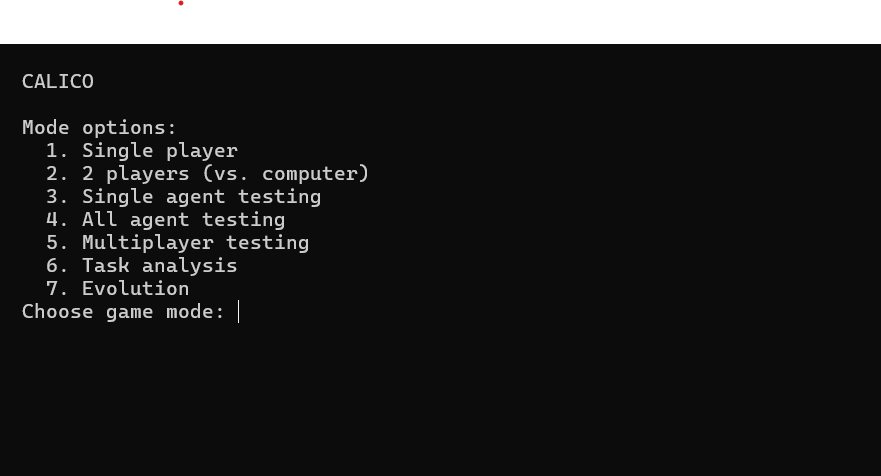
\includegraphics[width=8cm]{cs/obrazky/konzole.png}
    \caption{Konzole}
    \label{fig:konzole}
\end{figure}
}
\newcommand{\figureUkoly}{
\begin{figure}[H]
    \centering
    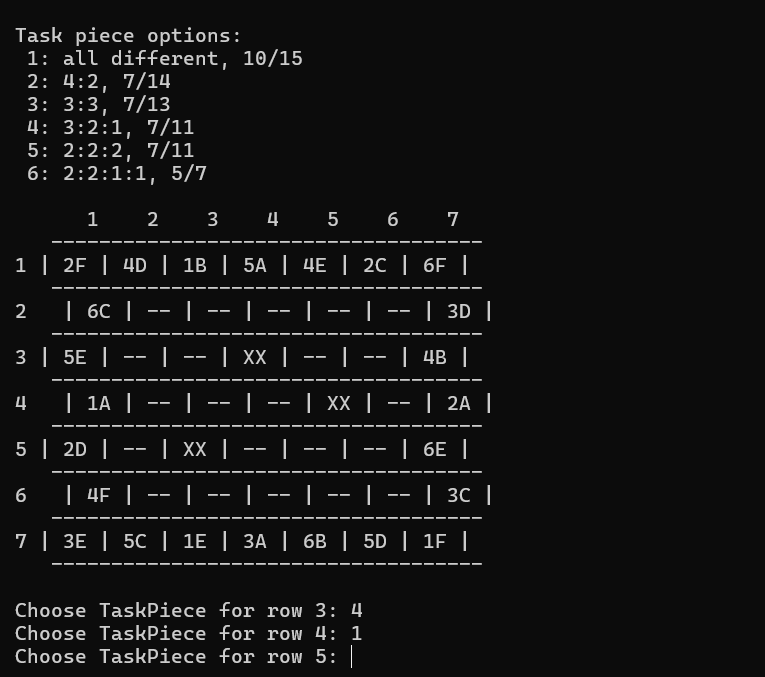
\includegraphics[width=8cm]{cs/obrazky/ukoly.png}
    \caption{Výběr úkolů na herní desku}
    \label{fig:ukoly}
\end{figure}
}
\newcommand{\figureSinglePlay}{
\begin{figure}[H]
    \centering
    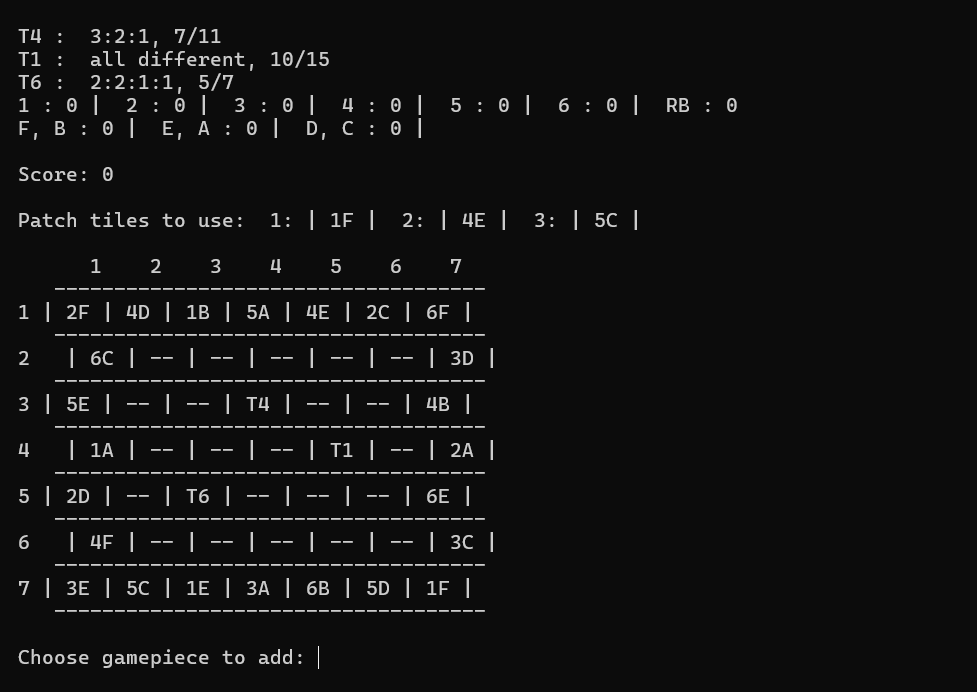
\includegraphics[width=8cm]{cs/obrazky/single.png}
    \caption{Stav hry pro jednoho hráče}
    \label{fig:singlePlay}
\end{figure}
}
\newcommand{\figureMultiPlay}{
\begin{figure}[H]
    \centering
    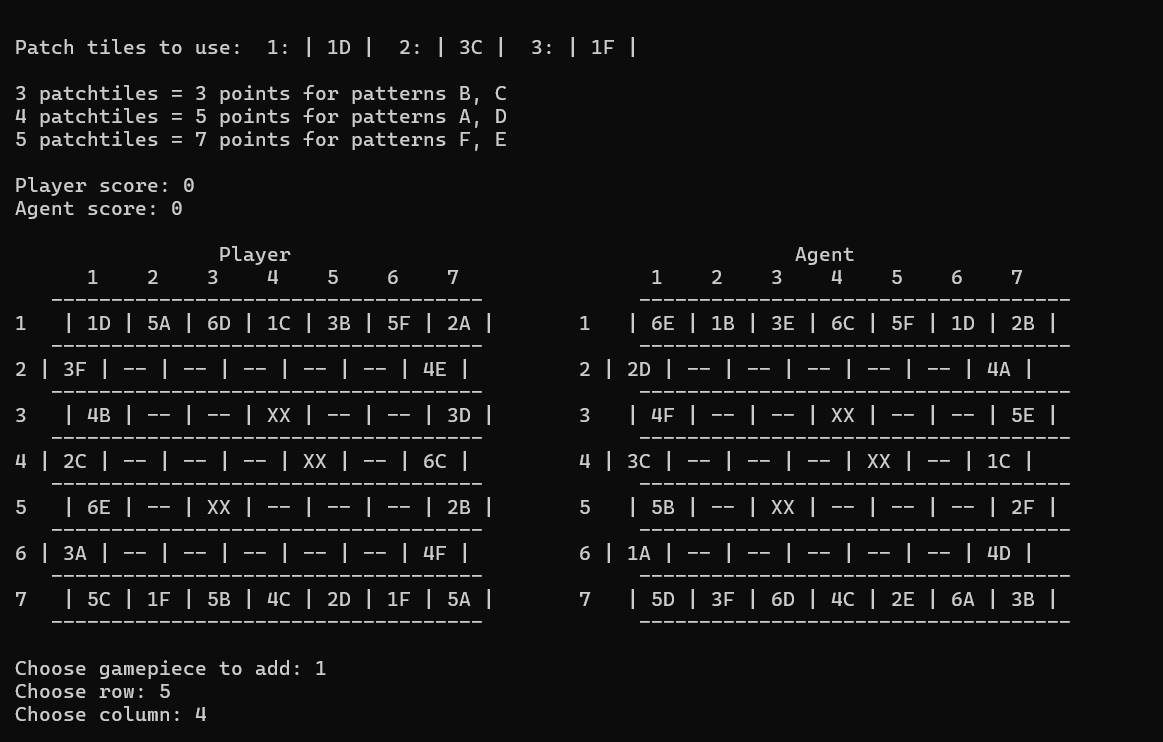
\includegraphics[width=8cm]{cs/obrazky/multi.png}
    \caption{Stav hry hráče proti počítači}
    \label{fig:multiPlay}
\end{figure}
}


\newcommand{\figureOmezeniHladovehoPristupuPriklad}{
\begin{figure}[H]
    \centering
    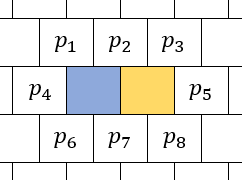
\includegraphics{cs/obrazky/stromoveProhledavaniPriklad.png}
    \caption{Příklad situace hry zjednodušené pouze na barvy dílků}
    \label{fig:omezeniHladovehoPristupuPriklad}
\end{figure}
}
\newcommand{\figureStrom}{
\begin{figure}[H]
    \centering
    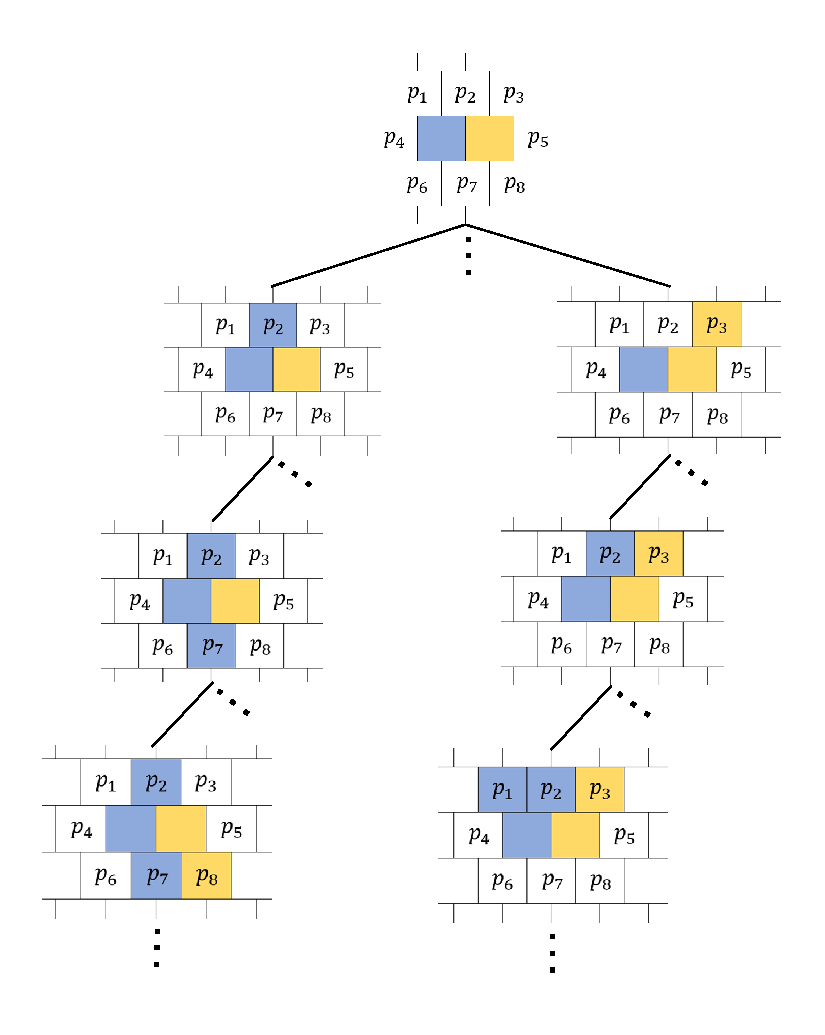
\includegraphics[width=10cm]{cs/obrazky/strom.pdf}
    \caption{Stromová reprezentace stavového prostoru}
    \label{fig:strom}
\end{figure}
}

\newcommand{\figureTS}{
\begin{figure}[H]
    \centering
    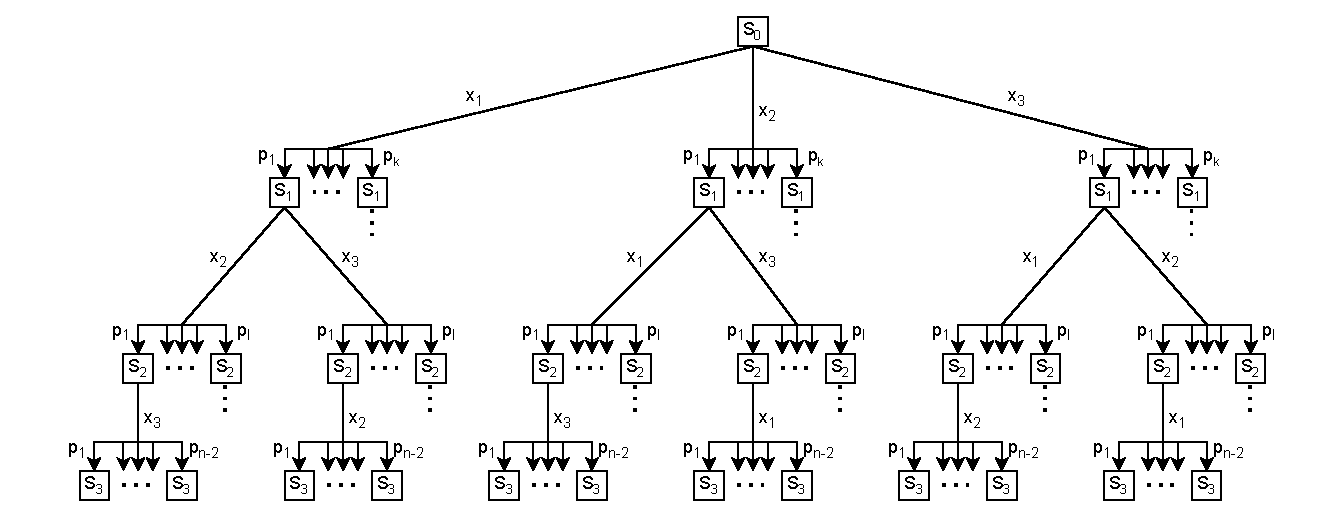
\includegraphics[width=14.7cm]{cs/obrazky/TS.pdf}
    \caption{Stromové prohledávání}
    \label{fig:TS}
\end{figure}
}

\newcommand{\figureMCTS}{
\begin{figure}[H]
    \centering
    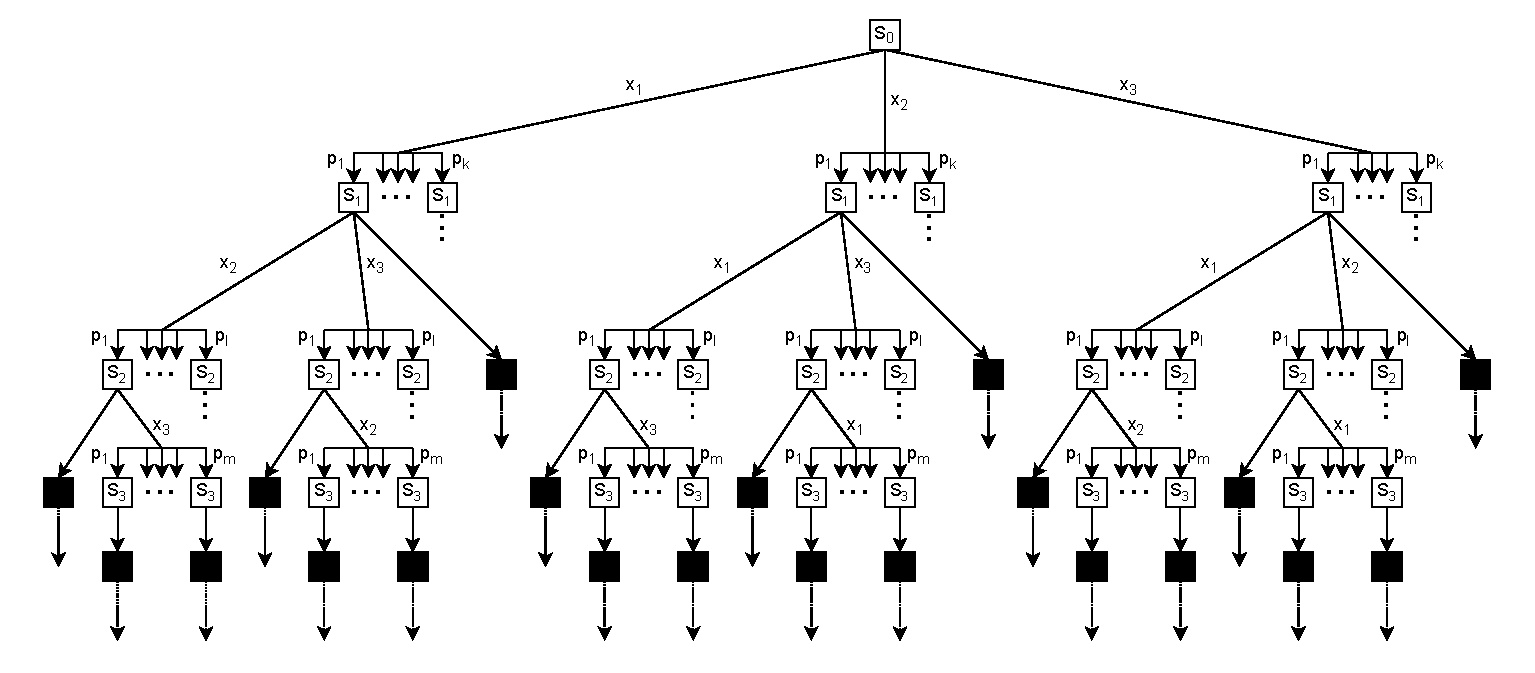
\includegraphics[width=14.7cm]{cs/obrazky/mc_tree.pdf}
    \caption{Stromové prohledávání inspirované MCTS}
    \label{fig:MCTS}
\end{figure}
}

\newcommand{\figureHerniDeska}{
\begin{figure}[H]
    \centering
    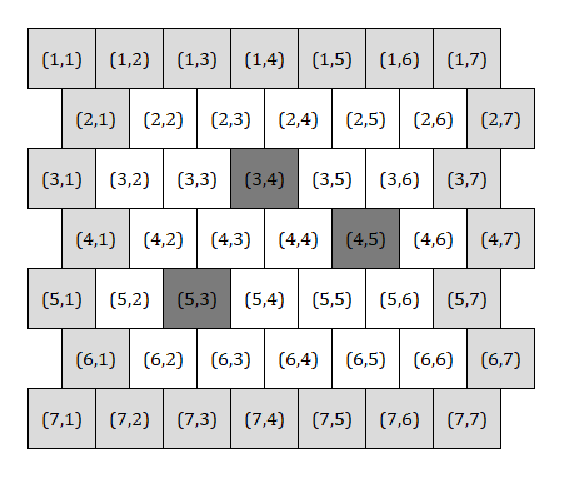
\includegraphics[width=7cm]{cs/obrazky/herniDeska.pdf}
    \caption{Reprezentace herní desky dvourozměrným polem}
    \label{fig:herniDeska}
\end{figure}
}

\newcommand{\figureZlepseniGraf}{
\begin{figure}[H]
    \centering
    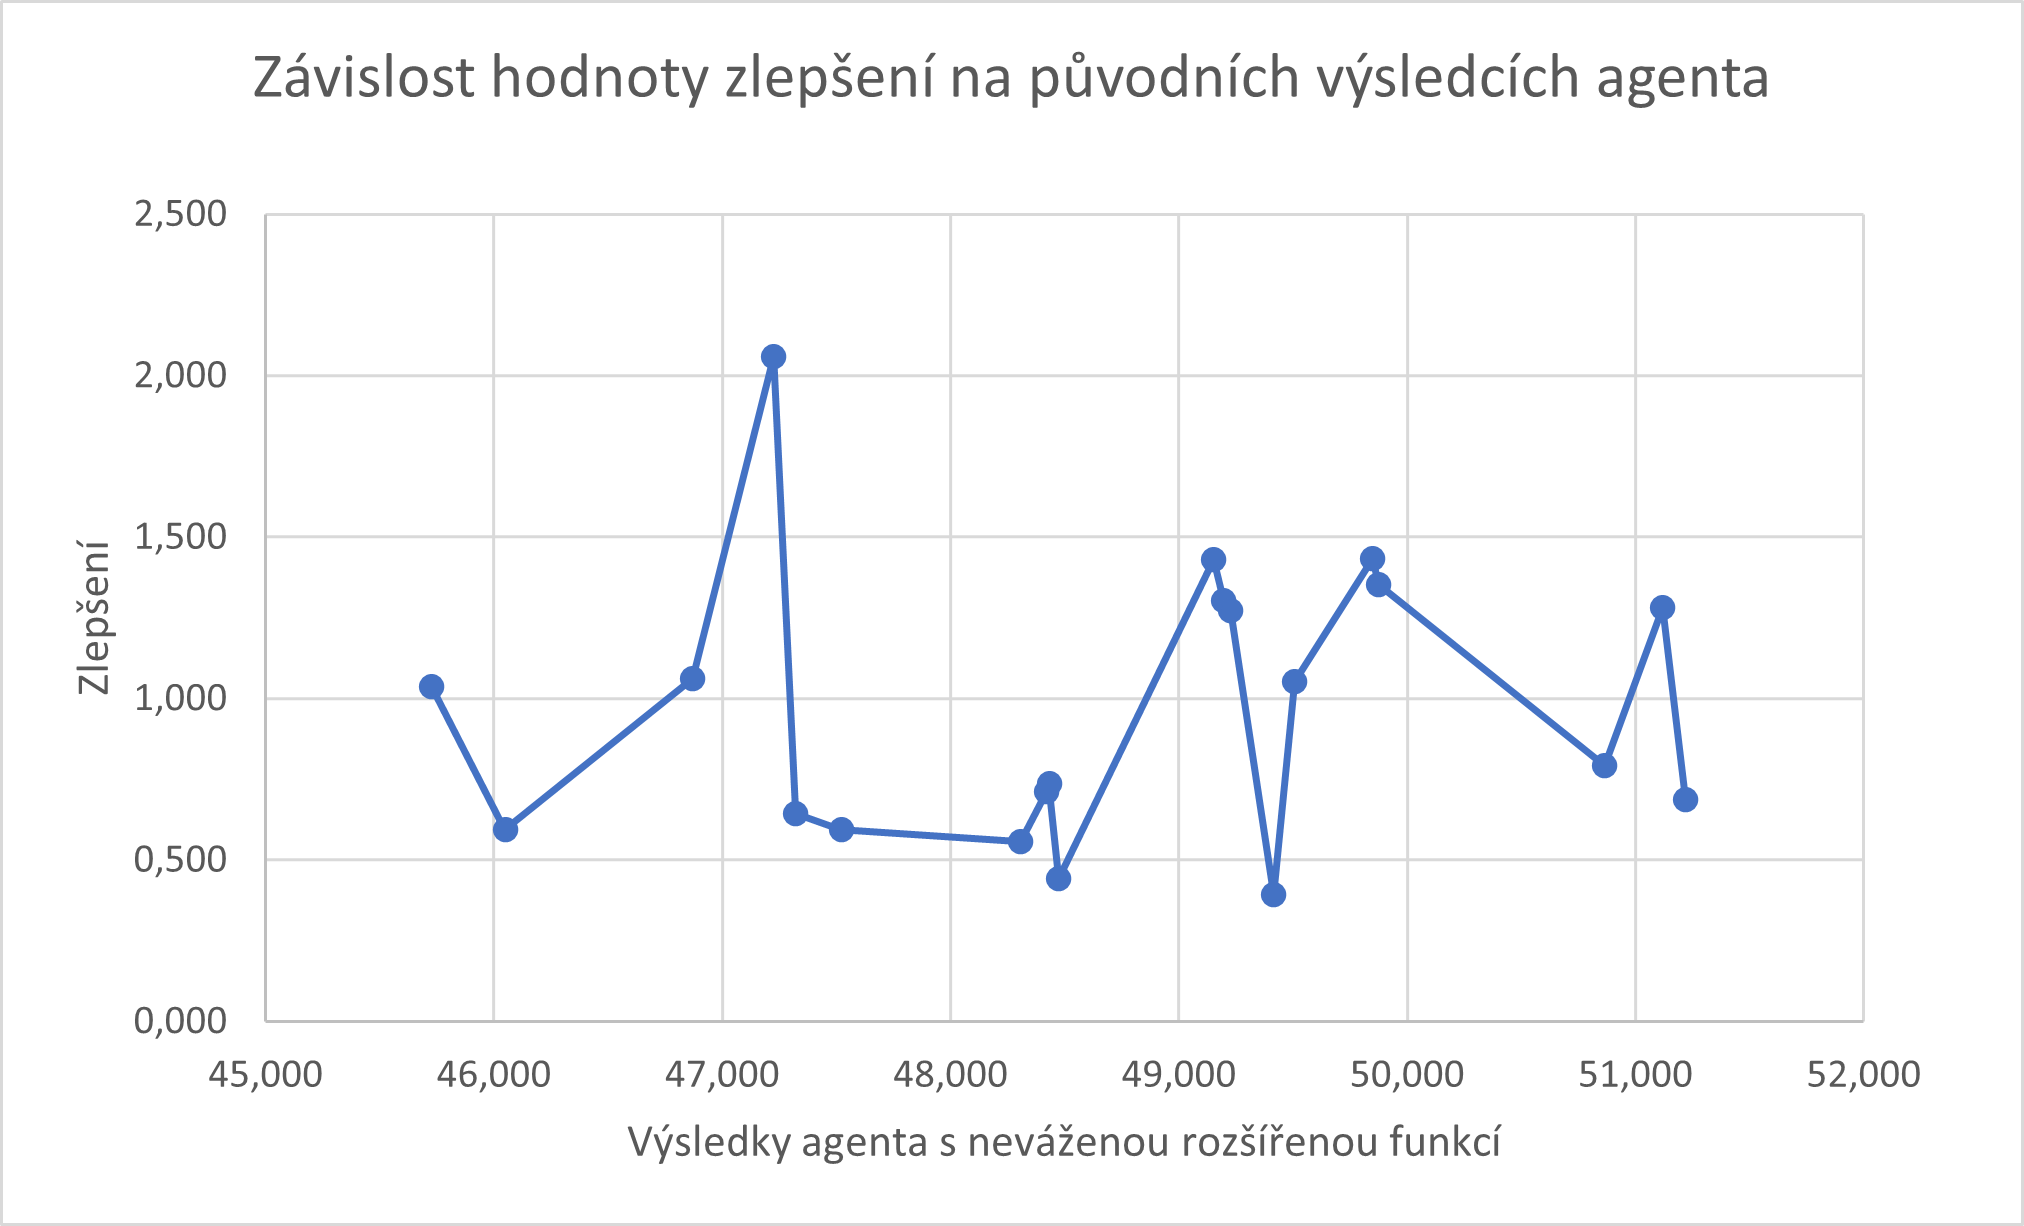
\includegraphics[width=10cm]{cs/obrazky/zavislostZlepseni.png}
    \caption{Graf závislosti}
    \label{fig:zlepseniGraf}
\end{figure}
}

\newcommand{\plotPokus}{
\begin{figure}[H]
\centering
\begin{tikzpicture}
\begin{axis}[
    scale only axis,
    height=5cm,
    width=10cm,
    xlabel={Průměrné skóre agenta s neváženou funkcí},
    ylabel={Zlepšení skóre},
    xmin=45, xmax=52,
    ymin=0, ymax=2.5,
    xtick={45,46,47,48,49,50,51,52},
    ytick={0.0,0.5,1.0,1.5,2.0,2.5},
    xmajorgrids=true,
    ymajorgrids=true,
    grid style=dashed,
]
\addplot[
    color=blue,
    mark=o,
    ]  
    coordinates {
    (45.726,1.038)
    (46.049,0.594)
    (46.872,1.060)
    (47.224,2.060)
    (47.323,0.642)
    (47.521,0.593)
    (48.307,0.556)
    (48.421,0.712)
    (48.432,0.738)
    (48.474,0.433)
    (49.151,1.430)
    (49.197,1.303)
    (49.228,1.274)
    (49.414,0.394)
    (49.509,1.052)
    (49.848,1.434)
    (49.874,1.352)
    (50.865,0.791)
    (51.120,1.283)
    (51.219,0.686)
    };
    
\end{axis}
\end{tikzpicture}
\caption{Graf závislosti zlepšení na původních výsledcích}
\label{graf}
\end{figure}

}


% Porovnání různých nastavení hry
\newcommand{\tableSettings}{
\begin{table}[H]
\centering
\small
\begin{tabular}{c|cccc|c} 
\hline
\textbf{Úkolové dílky} & \textbf{Deska 1} & \textbf{Deska 2} & \textbf{Deska 3} & \textbf{Deska 4} & \textbf{Průměr}  \\ 
\hline
2,3,5                  & 45,678           & 45,710           & 45,620           & 45,719           & 45,682           \\
1,2,3                  & 46,048           & 45,961           & 46,038           & 46,042           & 46,022           \\
2,3,6                  & 46,808           & 46,880           & 46,834           & 46,910           & 46,858           \\
2,3,4                  & 47,270           & 47,210           & 47,262           & 47,303           & 47,261           \\
1,3,5                  & 47,329           & 47,346           & 47,384           & 47,395           & 47,363           \\
1,2,5                  & 47,565           & 47,523           & 47,472           & 47,490           & 47,512           \\
1,3,6                  & 48,297           & 48,286           & 48,293           & 48,212           & 48,272           \\
3,5,6                  & 48,357           & 48,331           & 48,289           & 48,345           & 48,331           \\
1,2,6                  & 48,372           & 48,451           & 48,447           & 48,460           & 48,433           \\
2,5,6                  & 48,446           & 48,393           & 48,457           & 48,476           & 48,443           \\
3,4,5                  & 49,185           & 49,179           & 49,237           & 49,208           & 49,202           \\
1,3,4                  & 49,232           & 49,217           & 49,272           & 49,247           & 49,242           \\
2,4,5                  & 49,375           & 49,233           & 49,284           & 49,194           & 49,271           \\
1,5,6                  & 49,427           & 49,367           & 49,393           & 49,442           & 49,407           \\
1,2,4                  & 49,473           & 49,338           & 49,380           & 49,467           & 49,415           \\
3,4,6                  & 49,879           & 49,885           & 49,827           & 49,914           & 49,876           \\
2,4,6                  & 49,942           & 49,884           & 49,928           & 49,956           & 49,927           \\
1,4,5                  & 50,839           & 50,794           & 50,850           & 50,863           & 50,836           \\
4,5,6                  & 51,045           & 51,106           & 51,119           & 51,081           & 51,088           \\
1,4,6                  & 51,199           & 51,203           & 51,237           & 51,155           & 51,198           \\
\hline
\end{tabular}
\caption{Porovnání výsledků pro různá nastavení herní desky}
\label{tab:SettingsAll}
\end{table}
}

% Detailní porovnání nastavení s nejnižším skóre
\newcommand{\tableSettingsDetailWorst}{
\begin{table}[H]
\centering
\begin{minipage}{.3\linewidth}
\centering
\begin{tabular}{c c} 
\hline
\textbf{Úkoly} & \textbf{Skóre}  \\ 
\hline
2,3,5                  & 45,285                   \\
3,2,5                  & 45,619                   \\
2,5,3                  & 45,709                   \\
5,3,2                  & 45,812                   \\
5,2,3                  & 45,853                   \\
3,5,2                  & 45,858                   \\
\hline
\end{tabular}

\end{minipage}
\begin{minipage}{.3\linewidth}
\centering
\begin{tabular}{c c} 
\hline
\textbf{Úkoly} & \textbf{Skóre}  \\ 
\hline
2,3,1                  & 44,348                   \\
3,2,1                  & 44,614                   \\
2,1,3                  & 46,295                   \\
3,1,2                  & 46,459                   \\
1,2,3                  & 47,025                   \\
1,3,2                  & 47,133                   \\
\hline
\end{tabular}

\end{minipage}
\begin{minipage}{.3\linewidth}
\centering
\begin{tabular}{c c} 
\hline
\textbf{Úkoly} & \textbf{Skóre}  \\ 
\hline
2,6,3                  & 46,507                   \\
3,6,2                  & 46,735                   \\
2,3,6                  & 46,866                   \\
6,3,2                  & 46,951                   \\
3,2,6                  & 46,978                   \\
6,2,3                  & 47,194                   \\
\hline
\end{tabular}

\end{minipage}

\caption{Porovnání různých umístění kombinací s nejhoršími výsledky}
\label{tab:SettingsDetailWorst}
\end{table}
}

% Detailní porovnání nastavení s nejvyšším skóre
\newcommand{\tableSettingsDetailBest}{
\begin{table}[H]
\centering
\begin{minipage}{.3\linewidth}
\centering
\begin{tabular}{c c} 
\hline
\textbf{Úkoly} & \textbf{Skóre}  \\ 
\hline
4,5,1                  & 50,029                   \\
5,4,1                  & 50,064                   \\
4,1,5                  & 50,878                   \\
1,4,5                  & 51,135                   \\
5,1,4                  & 51,328                   \\
1,5,4                  & 51,754                   \\
\hline
\end{tabular}

\end{minipage}
\begin{minipage}{.3\linewidth}
\centering
\begin{tabular}{c c} 
\hline
\textbf{Úkoly} & \textbf{Skóre}  \\ 
\hline
6,4,1                  & 50,211                   \\
4,6,1                  & 50,588                   \\
6,1,4                  & 50,837                   \\
1,6,4                  & 51,710                   \\
4,1,6                  & 51,712                   \\
1,4,6                  & 51,850                   \\
\hline
\end{tabular}

\end{minipage}
\begin{minipage}{.3\linewidth}
\centering
\begin{tabular}{c c} 
\hline
\textbf{Úkoly} & \textbf{Skóre}  \\ 
\hline
6,5,4                  & 50,669                   \\
5,6,4                  & 50,829                   \\
6,4,5                  & 51,009                   \\
4,6,5                  & 51,098                   \\
4,5,6                  & 51,304                   \\
5,4,6                  & 51,370                   \\
\hline
\end{tabular}

\end{minipage}
\caption{Porovnání různých umístění kombinací s nejlepšími výsledky}
\label{tab:SettingsDetailBest}
\end{table}
}

% Porovnání jednokrokových agentů - skóre
\newcommand{\tableOneStepAgentsScore}{
\begin{table}[H]
\small
\centering
\begin{tabular}{l|c c c} 
\hline
\textbf{Agent} & \textbf{Průměrné skóre} & \textbf{Maximum} & \textbf{Minimum}  \\ 
\hline
RAND                 & 14,607                  & 45               & 0                 \\
základ - barvy       & 32,503                  & 62               & 15                \\
základ - vzory       & 31,305                  & 57               & 11                \\
základ - vše         & 45,338                  & 71               & 18                \\
rozšířená funkce     & \textbf{48,532}         & 71               & 20                \\
RAND s p=0,05       & 47,145                  & 71               & 20                \\
\hline
\end{tabular}
\caption{Porovnání výsledků jednokrokových agentů}
\label{tab:OneStepScores}
\end{table}
}

% Porovnání jednokrokových agentů - zisk žetonů
\newcommand{\tableOneStepAgentsDetailButtonsCats}{
\begin{table}[H]
\small
\centering
\begin{tabular}{l|cccc} 
\hline
\textbf{Agent}       & \textbf{Knoflíky} & \textbf{Kočky (3b.)} & \textbf{Kočky (4b.)} & \textbf{Kočky (5b.)}  \\ 
\hline
RAND                 & 2,375             & 0,821                & 0,264                & 0,083                 \\
základ - barvy       & 8,243             & 0,808                & 0,248                & 0,077                 \\
základ - vzory       & 2,308             & 2,743                & 1,386                & 0,792                 \\
základ - vše         & 6,532             & 2,147                & 0,908                & 0,390                 \\
rozšířená funkce     & 5,697             & 1,963                & 0,979                & 0,500                 \\
RAND s p=0,05      & 5,575             & 1,906                & 0,955                & 0,478                 \\
\hline
\end{tabular}
\caption{Porovnání počtu získaných žetonů jednokrokových agentů}
\label{tab:OneStepButtonsCats}
\end{table}
}

\newcommand{\tableOneStepAgentsDetailTasks}{
\begin{table}[H]
\small
\centering
\begin{tabular}{l|cccccc} 
\hline
\textbf{Agent} & \textbf{Úkol 1} & \textbf{Úkol 2} & \textbf{Úkol 3} & \textbf{Úkol 4} & \textbf{Úkol 5} & \textbf{Úkol 6}  \\ 
\hline
RAND                 & 0,040           & 0,018           & 0,009           & 0,277           & 0,077           & 0,708            \\
základ - barvy       & 0,022           & 0,015           & 0,015           & 0,354           & 0,143           & 0,737            \\
základ - vzory       & 0,016           & 0,040           & 0,032           & 0,451           & 0,104           & 0,647            \\
základ - vše         & 0,243           & 0,331           & 0,290           & 1,089           & 0,680           & 1,334            \\
rozšířená funkce     & 0,828           & 0,604           & 0,522           & 1,103           & 0,787           & 1,264            \\
RAND s p=0,05      & 0,799           & 0,572           & 0,487           & 1,097           & 0,746           & 1,260            \\
\hline
\end{tabular}
\caption{Porovnání počtu splněných úkolů pro jednokrokové agenty}
\label{tab:OneStepTasks}
\end{table}
}

% Porovnání stromového prohledávání pro 2 nebo 3 dílky  s různým discount factorem
\newcommand{\tableTreeSearchScoreTest}{
\begin{table}[H]
\centering
\begin{tabular}{l|cc} 
\hline
\multicolumn{1}{c|}{\textbf{Discount}} & \multicolumn{2}{c}{\textbf{Skóre}}                                \\
\multicolumn{1}{c|}{\textbf{faktor}}                                   & \textbf{Hloubka 2}                         & \textbf{Hloubka 3}                          \\ 
\hline
0,1                                & 50,685                     & 50,883                      \\
0,25                               & 51,061                     & 51,268                      \\
0,5                                & 51,497                     & 51,837                      \\
0,75                               & 51,781                     & 52,101                      \\
0,8                                & 51,734                     & 52,264                      \\
0,9                                & 51,647                     & 52,393                      \\
0,95                               & 51,699                     & 52,199                      \\
1                                  & 49,816                     & 49,315                      \\
\hline
\end{tabular}
\caption{Porovnání výsledků pro různé hodnoty discount faktoru a hloubky stromu}
\label{tab:testTS}
\end{table}
}

% Porovnání nejlepšího nastavení stromového prohledávání s jednokrokovým váženým rozšířeným ohodnocováním
\newcommand{\tableTreeSearchDetailScore}{
\begin{table}[H]
\centering
\small
\begin{tabular}{lccc} 
\hline
\textbf{Použití funkce} & \textbf{Skóre} & \textbf{Max} & \textbf{Min} \\ 
\hline
jednokrokově                    & 49,498               & 76              &  23                 \\
ve stromovém prohledávání       & 52,393               & 77              &  25                 \\
\hline
\end{tabular}
\caption{Porovnání skóre při použití vážené rozšířené funkce jednokrokově a ve stromovém prohledávání}
\label{tab:TSscore}
\end{table}
}

% Porovnání nejlepšího nastavení stromového prohledávání s jednokrokovým váženým rozšířeným ohodnocováním
\newcommand{\tableTreeSearchDetailButtonsCats}{
\begin{table}[H]
\centering
\footnotesize
\begin{tabular}{lcccc} 
\hline
\textbf{Použití funkce} & \textbf{Knoflíky} & \textbf{Kočky (3b.)} & \textbf{Kočky (4b.)} & \textbf{Kočky (5b.)}  \\ 
\hline
jednokrokově                    & 5,790                 & 2,093                     & 1,042                     & 0,528                      \\
ve stromovém prohledávání       & 6,065                 & 2,182                     & 1,125                     & 0,599                      \\
\hline
\end{tabular}
\caption{Porovnání počtu získaných žetonů při použití vážené rozšířené funkce jednokrokově a ve stromovém prohledávání}
\label{tab:TSZetony}
\end{table}
}

% Porovnání stromového prohledávání pro 2 nebo 3 dílky - úkoly
\newcommand{\tableTreeSearchDetailTasks}{
\begin{table}[H]
\centering
\footnotesize
\begin{tabular}{lcccccc} 
\hline
\textbf{Použití funkce} & \textbf{Úkol 1} & \textbf{Úkol 2} & \textbf{Úkol 3} & \textbf{Úkol 4} & \textbf{Úkol 5} & \textbf{Úkol 6}  \\ 
\hline
jednokrokově                             & 0,840           & 0,609           & 0,608           & 1,035           & 0,746           & 1,173                \\
ve stromovém prohledávání                & 0,863           & 0,635           & 0,640           & 1,105           & 0,830           & 1,259                \\
\hline
\end{tabular}
\caption{Porovnání splněných úkolů při použití vážené rozšířené funkce jednokrokově a ve stromovém prohledávání}
\label{tab:TSTasks}
\end{table}
}

% Porovnání MCTS pro různé počty simulací
\newcommand{\tableMCTSScore}{

\begin{table}[H]
\centering
\begin{tabular}{lllll} 
\hline
\textbf{Velikost simulace} & \textbf{Skóre} &\textbf{Max} &\textbf{Min} \\ 
\hline
5                          & 52,895         &  75         &  21                  \\
10                         & 55,404         &  75         &  29                  \\
25                         & 56,944         &  73         &  34                  \\
50                         & 57,312         &  72         &  37                  \\
75                         & 58,168         &  73         &  41                  \\
\hline
\end{tabular}
\caption{Porovnání výsledků pro různé počty her v simulaci}
\label{tab:MCTSSimulace}
\end{table}

}

% Porovnání MCTS pro různé omezení větvení pro 5 her v simulaci
\newcommand{\tableMCTSBranching}{
\begin{table}[H]
\centering
\begin{tabular}{lllll} 
\hline
\textbf{Omezení větvení} & \textbf{Skóre} &\textbf{Max} &\textbf{Min} \\ 
\hline
5                          & 52,895         &  75         &  21                  \\
max((prazdne+1)/2,5)       & 52,908         &  72         &  22                  \\

\hline
\end{tabular}
\caption{Porovnání výsledků pro různé omezení větvení}
\label{tab:MCTSBranching}
\end{table}
}

% Porovnání MCTS pro různé počty simulací
\newcommand{\tableMCTSDetailScore}{
\begin{table}[H]
\centering
\small
\begin{tabular}{lccc} 
\hline
\textbf{Stromové prohledávání} & \textbf{Skóre} & \textbf{Max} & \textbf{Min} \\ 
\hline
bez simulací                   & 52,393               & 77              &  25                 \\
se simulacemi                  & 58,168               & 73              &  41                 \\
\hline
\end{tabular}
\caption{Porovnání skóre pro stromové prohledávání}
\label{tab:MCTSscore}
\end{table}
}

% Porovnání MCTS pro různé počty simulací
\newcommand{\tableMCTSDetailButtonsCats}{
\begin{table}[H]
\centering
\footnotesize
\begin{tabular}{lcccc} 
\hline
\textbf{Stromové prohledávání} & \textbf{Knoflíky} & \textbf{Kočky (3b.)} & \textbf{Kočky (4b.)} & \textbf{Kočky (5b.)}  \\ 
\hline
bez simulací       & 6,065                 & 2,182                     & 1,125                     & 0,599                      \\
se simulacemi      & 6,656                 & 2,228                     & 1,312                     & 0,824                      \\
\hline
\end{tabular}
\caption{Porovnání počtu získaných žetonů pro stromové prohledávání}
\label{tab:MCTSZetony}
\end{table}
}

% Porovnání MCTS pro různé počty simulací
\newcommand{\tableMCTSDetailTasks}{
\begin{table}[H]
\centering
\footnotesize
\begin{tabular}{lcccccc} 
\hline
\textbf{Stromové prohledávání} & \textbf{Úkol 1} & \textbf{Úkol 2} & \textbf{Úkol 3} & \textbf{Úkol 4} & \textbf{Úkol 5} & \textbf{Úkol 6}  \\ 
\hline
bez simulací                & 0,863           & 0,635           & 0,640           & 1,105           & 0,830           & 1,259                \\
se simulacemi               & 0,835           & 0,608           & 0,545           & 1,444           & 1,035           & 1,504                \\
\hline
\end{tabular}
\caption{Porovnání splněných úkolů pro stromové prohledávání}
\label{tab:MCTSTasks}
\end{table}
}

% Porovnání vah pro různá umístění stejných tasků
\newcommand{\tableEvolDetail}{
\begin{table}[H]
\centering
\footnotesize
\begin{tabular}{c|c c c c c c c}
\hline
\multirow{2}{*}{\textbf{Úkoly}} & \multicolumn{7}{c}{\textbf{Váhy}} \\ 
& \textbf{Barva} & \textbf{Vzor(3b)} & \textbf{Vzor(4b)} & \textbf{Vzor(5b)} & \textbf{Úkol 1} & \textbf{Úkol 2} & \textbf{Úkol 4} \\ 
\hline
1,2,4                           & 0,933             & 1,129               & 0,998               & 0,990               & 1,218           & 1,134           & 0,597 \\
1,4,2                           & 0,976             & 1,152               & 1,027               & 1,031               & 1,077           & 1,098           & 0,640 \\
2,1,4                           & 0,971             & 1,220               & 1,073               & 1,024               & 1,109           & 1,055           & 0,548 \\
2,4,1                           & 0,985             & 1,213               & 1,017               & 0,927               & 1,173           & 1,113           & 0,572 \\
4,1,2                           & 0,955             & 1,190               & 1,020               & 0,997               & 1,153           & 1,115           & 0,571 \\
4,2,1                           & 0,895             & 1,167               & 1,052               & 0,964               & 1,186           & 1,097           & 0,639 \\
\hline
\end{tabular}
\caption{Výsledné váhy pro kombinaci úkolů 1, 2 a 4}
\label{tab:evolDetail124}
\end{table}
}

\newcommand{\tableEvolDetailTwo}{
\begin{table}
\centering
\begin{tabular}{c|c c c c c c c} 
\hline
\multirow{2}{*}{\textbf{Úkoly}} & \multicolumn{7}{c}{\textbf{Váhy}}                                                                                                 \\
                                & \textbf{Barva} & \textbf{Vzor(3b)} & \textbf{Vzor(4b)} & \textbf{Vzor(5b)} & \textbf{Úkol 1} & \textbf{Úkol 5} & \textbf{Úkol 6}  \\ 
\hline
1,5,6                           & 1,038          & 1,154             & 1,083             & 0,999             & 1,159           & 0,924           & 0,643            \\
1,6,5                           & 0,929          & 1,133             & 0,972             & 0,934             & 1,155           & 1,002           & 0,875            \\
5,1,6                           & 1,073          & 1,059             & 1,000             & 0,962             & 1,346           & 0,898           & 0,661            \\
5,6,1                           & 0,894          & 1,126             & 1,045             & 0,899             & 1,113           & 1,052           & 0,870            \\
6,1,5                           & 1,064          & 0,987             & 0,941             & 0,877             & 1,249           & 1,059           & 0,823            \\
6,5,1                           & 1,018          & 0,999             & 1,021             & 0,974             & 0,995           & 0,942           & 1,051            \\
\hline
\end{tabular}
\caption{Výsledné váhy pro kombinaci úkolů 1, 5 a 6}
\end{table}
}

% Porovnání skóre s váženou ohodnocující fcí proti nevážené fci
\newcommand{\tableEvolScore}{
\begin{table}[H]
\centering
\begin{tabular}{c|l|l|l} 
\hline
\textbf{Úkolové dílky} & \textbf{Nevážená funkce} & \textbf{Vážená funkce} & \textbf{Zlepšení}  \\ 
\hline
1,2,3                  & 46,049                   & 46,643                 & 0,594              \\
1,2,4                  & 49,509                   & 50,561                 & 1,052              \\
1,2,5                  & 47,521                   & 48,113                 & 0,593              \\
1,2,6                  & 48,474                   & 48,916                 & 0,443              \\
1,3,4                  & 49,228                   & 50,501                 & 1,274              \\
1,3,5                  & 47,323                   & 47,965                 & 0,642              \\
1,3,6                  & 48,307                   & 48,863                 & 0,556              \\
1,4,5                  & 50,865                   & 51,656                 & 0,791              \\
1,4,6                  & \textbf{51,219}          & 51,905                 & 0,686              \\
1,5,6                  & 49,414                   & 49,808                 & 0,394              \\
2,3,4                  & 47,224                   & 49,284                 & \textbf{2,060}     \\
2,3,5                  & 45,726                   & 46,764                 & 1,038              \\
2,3,6                  & 46,872                   & 47,932                 & 1,060              \\
2,4,5                  & 49,197                   & 50,501                 & 1,303              \\
2,4,6                  & 49,848                   & 51,282                 & 1,434              \\
2,5,6                  & 48,432                   & 49,170                 & 0,738              \\
3,4,5                  & 49,151                   & 50,581                 & 1,430              \\
3,4,6                  & 49,874                   & 51,227                 & 1,352              \\
3,5,6                  & 48,421                   & 49,133                 & 0,712              \\
4,5,6                  & 51,120                   & \textbf{52,403}        & 1,283              \\ 
\hline
\textbf{průměr}        & \textbf{48,689}          & \textbf{49,660}        & \textbf{0,972} \\
\hline
\end{tabular}
\caption{Výsledky vážené funkce pro jednotlivé kombinace úkolů}
\label{tab:weightedScoreAll}
\end{table}
}

\newcommand{\tableWeightedDetailScore}{
\begin{table}[H]
\centering
\small
\begin{tabular}{lccc} 
\hline
\textbf{Rozšířená funkce} & \textbf{Skóre} & \textbf{Max} & \textbf{Min} \\ 
\hline
nevážená                & 48,532         & 71               & 20                 \\
vážená                  & 49,498         & 76               & 23                 \\
\hline
\end{tabular}
\caption{Porovnání skóre pro váženou funkci}
\label{tab:weightedScore}
\end{table}
}

% Porovnání MCTS pro různé počty simulací
\newcommand{\tableWeightedDetailButtonsCats}{
\begin{table}[H]
\centering
\footnotesize
\begin{tabular}{lcccc} 
\hline
\textbf{Rozšířená funkce} & \textbf{Knoflíky} & \textbf{Kočky (3b.)} & \textbf{Kočky (4b.)} & \textbf{Kočky (5b.)}  \\ 
\hline
nevážená       & 5,697             & 1,963                & 0,979                & 0,500                      \\
vážená         & 5,790                 & 2,093                     & 1,042                     & 0,528                      \\
\hline
\end{tabular}
\caption{Porovnání počtu získaných žetonů pro váženou funkci}
\label{tab:weightedZetony}
\end{table}
}

% Porovnání MCTS pro různé počty simulací
\newcommand{\tableWeightedDetailTasks}{
\begin{table}[H]
\centering
\footnotesize
\begin{tabular}{lcccccc} 
\hline
\textbf{Rozšířená funkce} & \textbf{Úkol 1} & \textbf{Úkol 2} & \textbf{Úkol 3} & \textbf{Úkol 4} & \textbf{Úkol 5} & \textbf{Úkol 6}  \\ 
\hline
nevážená                & 0,828           & 0,604           & 0,522           & 1,103           & 0,787           & 1,264                \\
vážená                  & 0,840           & 0,609           & 0,608           & 1,035           & 0,746           & 1,173                \\
\hline
\end{tabular}
\caption{Porovnání splněných úkolů pro váženou funkci}
\label{tab:weightedTasks}
\end{table}
}

% Deviation pro různé počty her
\newcommand{\tableDeviation}{
\begin{table}[H]
\centering
\begin{tabular}{cc}
\hline
\textbf{Počet her} & \textbf{Odchylka v průměrných výsledcích}  \\
\hline
100       & 0,733                \\
250       & 0,448                \\
500       & 0,336                \\
750       & 0,252                \\
1000      & 0,224                \\
2500      & 0,140                \\
5000      & 0,106              \\
\hline
\end{tabular}
\caption{Odchylky od průměrného skóre pro různé počty her}
\label{tab:deviation}
\end{table}
}


\nocite{*}

%%% Jednotlivé kapitoly práce jsou pro přehlednost uloženy v samostatných souborech
\chapter*{Úvod}
\addcontentsline{toc}{chapter}{Úvod}

Calico je desková hra pro 1-4 hráče vydaná v roce 2020. Pro sólovou verzi hry vznikla webová aplikace \citep{calicoGame} a na jaře roku 2024 byla vydaná počítačová implementace na herní platformě Steam \citep{quiltsAndCatsOfCalico}. Tato implementace již podporuje hru pro více hráčů, avšak pouze online proti jiným lidským hráčům, neimplementuje žádného počítačového agenta. Pro hru Calico zatím nebyla provedena žádná analýza strategií ani samotného nastavení hry.

V této práci se nejprve seznámíme s pravidly hry a popíšeme vlastnosti její sólové verze. Dále se budu zaměříme na různé strategie, které lze využít při implementaci počítačového agenta. Při implementaci strategií využijeme různé přístupy z oblasti teorie her a umělé inteligence a tyto přístupy vzájemně porovnáme. Cílem práce je nalézt co nejlepší strategii pro sólovou verzi hry, kterou pak bude možné využít i pro hru lidského hráče proti počítači. Také porovnáme různé možnosti počátečního nastavení hry a jejich vliv na dosažitelnost vyššího finálního skóre.

Pro účely testování jsem vytvořila počítačovou implementaci hry v jazyce C\#, která je ovládaná konzolově.






%%% Fiktivní kapitola s ukázkami sazby

\chapter{Popis hry}

Hra Calico je založena na principu postupného přikládání dílků. 

Každý hráč má vlastní herní desku s políčky v mřížce velikosti 5$\times$5 z nichž 3 políčka jsou určena pro speciální dílky rozšíření hry. Na desku postupně doplňuje dílky s různými barvami a vzory a získává body podle zadaných pravidel na seskupování barev a vzorů v mřížce. Hráči se při vybírání dílků střídají. Hra končí, když mají všichni hráči vyplněné celé herní pole.

Vítězí hráč, kterému se podaří získat nejvíce bodů.
\todo[inline,color=red!40]{Možná trochu upravit - pročíst!}

\section{Pojmy}

\todo[inline]{Nějaká věta že pojmy}

\begin{itemize}
    \item Útržky - šestiúhelníkové dílky, které hráči pokládají na své herní desky. Každý útržek má svou barvu a vzor. Hra obsahuje 3 útržky pro každou kombinaci 6 barev a 6 vzorů, tedy 108 útržků.
    \item Úkolový dílek - Úkolové dílky se přikládají na 3 speciálně určená místa na hrací desce. Specifikují podmínky pro přikládání útržků na pozice s úkolovým dílkem sousedící hranou. Hráč tyto podmínky nemusí splnit, ovšem za~jejich splnění získává body.
    \item Dílky vzorů - Dílky vzorů jsou černobílé útržky, pro každý vzor existuje právě jeden. Slouží k určení bodování pro jednotlivé vzory. Přikládají se k panelům koček.
    \item Panel kočky - Panel kočky je karta, která slouží k určení bodování pro jednotlivé vzory. Každý panel určuje podmínku sdružování vzorů a odpovídající bodové ohodnocení. Podmínka je buď minimální počet sousedících útržků stejného vzoru, nebo přímo tvar, který mají útržky tvořit. K panelům koček se přikládají dílky vzorů.
    \item Pelíšek - Jako pelíšek je označena souvislá plocha útržků se stejným vzorem splňující minimální počet útržků podle odpovídajícího panelu kočky.
    \item Žeton kočky - Žetony s obrázky koček sloužící k~označování částí hrací desky, za které hráči získávají body. Přikládají se na již přiložené útržky.
    \item Přilákání kočičky - Hráč kočičku přiláká tím, že splní podmínky panelu kočky. Poté si na hrací desku přidá žeton kočky, který danému panelu odpovídá.
    \item Knoflík - Knoflíky jsou barevné žetony v barvách útržků, které slouží k~označování částí hracího pole, za které hráči získávají body. Přikládají se na již přiložené útržky.
    \item Duhový knoflík - Duhový knoflík je žeton, který hráč získá, pokud získá knoflík pro každou ze 6 barev.
\end{itemize}

\section{Základní pravidla}

\subsubsection*{Začátek hry}

Každý hráč dostane svou hrací desku a stejnou sadu 6 úkolových dílků. Na políčka pro úkolové dílky hráč položí 3 úkolové dílky dle svého výběru. 
Na stůl se položí 3 panely koček - pro seskupení 3 a více, 4 a více a 5 a více stejně vzorovaných dílků bez přesně určeného tvaru seskupení. Každému panelu kočky náhodně přidělíme 2 černobílé dílky vzorů. 
Bank knoflíků a kočiček podle použitých panelů necháme v dosahu všech hráčů. 
Všechny útržky se vloží do sáčku a zamíchají. Každý hráč si vezme 2 útržky ze sáčku a vezme si je do ruky, ostatním je neukazuje. Na stůl se vyloží nabídka 3 útržků.

\subsubsection*{Průběh hry}

V každém kole hry se všichni hráči vystřídají na tahu ve stejném na začátku stanoveném pořadí. Hráč na tahu vybere 1 z dílků, které má v ruce, a přidá ho na svou hrací desku na libovolné neobsazené políčko. Pokud má nárok na knoflík nebo kočičku, položí dané žetony na svou hrací plochu podle pravidel přikládání žetonů. Poté si vezme do ruky dílek z banku a bank doplní útržkem z pytlíku.

%\subsubsection*{Pravidla pro získání a přikládání žetonů}
\subsubsection*{Bodování knoflíků}
Za každý knoflík hráč získá 3 body. Knoflíků stejné barvy může hráč získat víc, nově vzniklá plocha alespoň 3 útržků však musí být oddělená od ploch, za které již hráč knoflík této barvy získal. Pokud hráč během hry spojí více ploch, na které již knoflíky umístil, dané knoflíky mu zůstávají.

\subsubsection*{Bodování koček}
Panely koček jsou ohodnoceny 3, 5 a 7 body.
Pro přilákání kočiček platí podobná pravidla jako pro knoflíky, pro přilákání kočičky vzorem, pro který jsme již vytvořili pelíšek, je potřeba vytvořit plochu, která s daným pelíškem nesousedí. Dva pelíšky různých vzorů ze stejného panelu kočky však sousedit mohou. \todo[inline,color=red!40]{přepsat}

\subsubsection*{Bodování úkolových dílků}
Úkolové dílky mají dvě možnosti bodového ohodnocení - za částečné a úplné splnění. Částečné splnění znamená splnění podmínky pouze vzorem nebo pouze barvou, úplné splnění pak znamená splnění podmínky barvou i vzorem. Každý úkolový dílek má jiné bodové ohodnocení, které je specifikováno přímo na dílku.


\subsubsection*{Konec hry}

Hra končí, když všichni hráči naplní celé své hrací desky, tedy po 22 kolech. Vyhrává hráč s~nejvyšším součtem bodů. Hra nabízí více verzí, které je také možné kombinovat s dalšími možnostmi rozšíření.


\section{Varianty hry a možná rozšíření}

Pravidla popsaná v předchozí sekci platí pro základní hru ve zjednodušeném režimu.

\subsubsection*{Základní pravidla v plné verzi}
Tato verze nabízí hráčům volbu panelů koček. Hráči tedy můžou volit mezi více možnostmi podmínek pro shlukování vzorů. Panely se složitějšími podmínkami jsou ohodnoceny více body.

\subsubsection*{Sólová hra}
Všechny varianty lze hrát ve verzi pro jednoho hráče, avšak absence protihráčů způsobuje nepříliš velkou obměnu možností útržků. Sólová varianta hry tento aspekt řeší tím, že po každém svém tahu hráč zahodí ten útržek z banku možností, který je více vpravo. Tuto verzi implementuje webová aplikace \citep{calicoGame}.

\subsubsection*{Další možné úpravy}
Hráči mohou dalšími možnostmi úprav měnit náročnost hry. Pro jednodušší hru je možné využít tzv. rodinnou verzi, ve které hráči neplní úkoly. Na začátku hry si na pole herní desky, které jsou určená pro úkolové dílky, položí úkolové dílky lícem dolů. Na tato místa se tedy nedají přikládat hrací dílky a počet kol zůstává oproti běžné verzi stejný. Pro snížení počtu dílků ve hře je možné odstranit jednu barevnou sadu dílků (36 dílků). Hráči se však také mohou domluvit na zpřísňujících pravidlech pro hru jako jsou např. různá omezení pro počet získaných knoflíků a žetonů koček.

Dále také mohou hráči upravovat herní mechaniky. Jako příklad lze uvést hru, ve které hráči nemají žádné útržky v ruce, ale ve svém tahu přikládají na svou herní desku přímo dílek z trojice dílků uprostřed stolu. Každý tah hráče pak může být omezen pravidlem, že pokud je to možné, musí přiložit takový dílek, který lze přiložit k dílku stejné barvy nebo stejného vzoru.

\begin{itemize}
    \item plnění milníků při více hrách za sebou, např. hráč nesmí za 1 hru získat žádný knoflík, hráč musí získat po 2 žetonech každé kočky ve hře, hráč musí získat více než určený počet bodů
\end{itemize}

\section{Implementované změny}

používám základní hru ve zjednodušeném režimu spolu s rozšířením, ve kterém hráči nemají dílky v ruce, ale přikládají rovnou dílek ze tří možností na stole

automatické počítání bodů v průběhu hry -> neřeším pravidla pokládání žetonků na herní desku


\chapter{Analýza hry}

\section{Vlastnosti hry}

Pro verzi hry pro jednoho hráče je důležitá vlastnost konečnosti, hra má předem daný počet tahů, které hráč může provést, který odpovídá počtu volných políček na herní desky. Hráč má tedy v průběhu hry k dispozici 22 tahů.

Nabídka herních dílků pro každý tah není předem známý, hráč tedy zná všechny proveditelné kroky pouze pro aktuální tah. 

Ve verzi pro více hráčů se mnou implementovaným rozšířením se jedná o hru s úplnou informací, to znamená, že všichni hráči mají stejné informace o hře. Pro strategii hráčů to znamená, že mohou uvažovat i akce, které ublíží jejich protihráčům.

Hra je sekvenční, tedy v každém kole se na tahu hráči vystřídají v předem stanoveném pořadí. 

Calico je hra s nenulovým součtem, což znamená, že zisky a ztráty jednotlivých hráčů nejsou přesně vyvážené. Zisk bodů jednoho hráče neznamená, že jiný hráč o body přichází.

\textbf{Vzájemná interakce hráčů ve hře}


\section{Herní strategie}

Strategie hráče definuje jeho rozhodování, kterou akci provést ve jakémkoliv stavu hry. Strategie ve stavu hry je funkce, která vrací akce, které hráč může v daném stavu provést v souladu s jeho strategií.


\subsection{Hladový přístup}

Agent v každém kroku hry vybere nejlepší právě teď, nezohledňuje, jak daná akce ovlivní další akce. V každém kroků tedy vybíráme lokálně nejlepší možnost, tím se však můžeme připravit o vyšší výsledné skóre ve hře.

\subsection{Stromová reprezentace hry}

Stavový prostor hry lze reprezentovat stromovým grafem. Vrcholy grafu odpovídají různým stavům hry a hrany mezi vrcholy odpovídají akcím, kterými lze mezi vrcholy přecházet. 

Stromová reprezentace hry je často používaná zejména u her pro 2 hráče, kteří se střídají na tahu. Akce hráčů se střídají po hladinách. Na obrázku xy můžeme vidět část stromové reprezentace hry TicTacToe. Listy stromu odpovídají koncovým stavům, tedy stavům, na které již nelze aplikovat žádné akce. Při dosažení koncového stavu je každému hráči přiděleno ohodnocení, které odpovídá jeho zisku nebo ztrátě ve hře (jeho herní výsledek). Takové ohodnocení může být ukazatelem prohry/výhry nebo počtem bodů, kterého hráč ve hře dosáhl. \citep{millington2016artificial}

Stromovou reprezentaci lze však využít i pro hru jednoho hráče. Pro aktuální stav vybudujeme stromovou reprezentaci možných budoucích kroků a zvolíme takovou posloupnost akcí, která vede k nejlépe ohodnocenému koncovému stavu. 

Jeden z největších problémů této reprezentace je velikost stavového prostoru. Stavy hry se mohou ve stromu opakovat. Pro stavy s mnoha aplikovatelnými akcemi vzniká velké větvení stromu. Pro hry, které nemají pevně daný počet kroků, které agent vykoná, můžeme dostat strom s velkou nebo dokonce nekonečnou hloubkou. Vyhodnocení takového stromu tedy bude prostorově i časově náročné.

Velké větvení i hloubku stromu lze omezit pomocí heuristické funkce, pomocí které ohodnotím každý vrchol stromu tak, aby ohodnocení odpovídalo tomu, nakolik přechod do daného stavu přispěje k výsledku hráče. Pomocí této heuristiky můžeme předpovídat, které větve pravděpodobněji dosáhnou lepších výsledků, a na základě toho zahazovat ostatní větve. Tento přístup je označován jako ořezávání stromu. Dále je s touto heuristikou možné omezit hloubku stromu na pevně daný počet kroků a místo ohodnocení koncového stavu použít pro vyhodnocení větve hodnotu heuristické funkce. Tento přístup může výrazně zlepšit složitost vyhodnocení strategie hráče, ovšem můžeme v rámci ořezávání přijít o nejlepší řešení.



\subsection{Monte Carlo Tree Search}

Monte Carlo Tree Search (MCTS) je heuristický prohledávací algoritmus často užívaný v rozhodovacích procesech, zejména v teorii her a jiných úlohách, kdy je potřeba prohledávat velký stavový prostor. Algoritmus je schopný provádět informovaná rozhodnutí i v komplexním prostředí s velkou mírou nejistoty.

MCTS využívá metodu Monte Carlo, která pomocí samplování náhodných vzorků z  určité pravděpodobnostní distribuce a využití statistiky vytváří odhady kvantit, které je náročné spočítat. Kromě teorie her se tato metoda využívá např. pro výpočet vícerozměrných integrálů. Ve stromovém prohledávání je tato metoda užitečná pro rozhodování, které stavy je výhodnější prohledávat.

Algoritmus MCTS opakuje následující 4 kroky po předem určenou dobu, nebo dokud nedojde ke splnění nějaké podmínky.

V prvním kroku pomocí heuristické strategie určíme, který vrchol budeme dále prohledávat. Nejběžnější strategií je Upper Confidence Bound for Trees (UCT), která kombinuje hodnotu vrcholu získanou z náhodných simulací následujících kroků a počet navštívení daného vrcholu v průběhu iterací algoritmu. Lze ji vyjádřit následující funkcí:
\begin{equation}
    S_i = x_i + c \cdot \sqrt{\frac{\ln(t)}{n_i}}
\end{equation}
kde $x_i$ je hodnota vrcholu, $c$ konstanta, $t$ počet iterací algoritmu, $n_i$ počet navštívení vrcholu.

V následujícím kroku vybraný vrchol rozšíříme o potomka.

Pro potomka provedeme simulaci, tedy simulujeme posloupnost náhodných kroků dokud nedojdeme k cíli, nebo nesplníme jiný požadavek k zastavení simulaci (např. pevně určený počet kroků). Hodnota vrcholu je určena hodnotou ze simulace.

Po získaní hodnoty ze simulace aktualizujeme hodnoty všech vrcholů na cestě ke kořeni zpětnou propagací.


\subsection{Evoluční algoritmus}

Následující text vznikl podle textu \citep{pilatEvolucniAlgoritmy}.
Evoluční algoritmy jsou optimalizační algoritmy inspirované biologickou evolucí. Pracujeme s množinou kandidátů na řešení daného problému, těmto kandidátům říkáme jedinci a množinu jedinců označujeme jako populaci. 

Jedna iterace evolučního algoritmu se nazývá generace. V každé generaci algoritmu vyhodnotíme tzv. fitness funkci každého jedince, která určuje, nakolik je řešení problému reprezentované daným jedincem dobré. Generace se typicky skládá z následujících částí.

\subsubsection*{Selekce}

Z aktuální populace potřebujeme vybrat jedince, ze kterých následně vytvoříme jedince pro novou generaci. Takovým jedincům říkáme rodiče, nové populaci pak jejich potomci. Příkladem může být turnajová selekce, kde s pravděpodobností $p_t$ z několika náhodně vybraných jedinců vybereme jako rodiče toho, který má nejlepší hodnotu fitness. 

\subsubsection*{Genetické operátory}

Na rodiče vybrané z aktuální generace dále aplikujeme genetické operátory. 
Operace křížení kombinuje dva jedince pro vytvoření jedince nového. Příkladem může být jednobodové křížení, kde náhodně vybereme jeden bod v jedinci. Potomek pak vznikne spojením dvou částí různých jedinců (rodičů) rozdělených daným bodem. 
Operace mutace vytvoří nového jedince tím, že náhodně upraví některé parametry již existujícího jedince, např. vygeneruje náhodnou novou hodnotu pro jeden z evolvovaných parametrů nebo prohodí hodnoty na dvou pozicích. Lze rozlišit mutaci zatíženou, která upravuje stávající hodnoty, a mutace nezatížené, které stávající hodnoty nijak nezohledňují.
\chapter{Reprezentace herního pole}

Pro implementaci hry je potřeba reprezentovat herní pole. Herní dílky mají šestiúhelníkový tvar, herní pole se tedy skládá z šestiúhelníkových políček. Potřebujeme tedy v reprezentaci zachovat to, že každá pozice sousedí se 6 dílky. Pro takovou reprezentaci využijeme dvojrozměrné pole, ve kterém budeme souřadnice sousedních dílků určovat zvlášť pro liché a sudé řádky. Množiny sousedních pozic pro pozici $(i,j)$ jsou vyjádřeny následovně:
\begin{align*}
    &\text{liché $i$: } \{(i-1,j-1),(i-1,j),(i,j-1),(i,j+1),(i+1,j-1),(i+1,j)\}\\
    &\text{sudé $i$: } \{(i-1,j),(i-1,j+1),(i,j-1),(i,j+1),(i+1,j),(i+1,j+1)\}
\end{align*}

Dvourozměrné pole s tímto výpočtem sousednosti lze vyjádřit obrázkem \ref{fig:herniDeska}. Výpočtem jsme tedy vytvořili jakési posunutí sudých řádků, tedy každé políčko herního pole, které není krajní, má 6 sousedních pozic. Pro krajní políčka nemusíme funkci na výpočet sousednosti měnit, jelikož množinu sousedů využijeme pouze při vyhodnocení přidání dílku na danou pozici, což se krajních polí netýká, jelikož jsou na začátku hry již obsazené předem určenými herními dílky.

\figureHerniDeska

Světle šedá políčka tedy značí pozice, které jsou předvyplněné a v průběhu hry na ně nelze přidávat herní dílky. Tmavě šedou barvou jsou označena políčka, na které hráč na začátku hry umístí úkolové dílky.



\chapter{Implementace agentů}

\section{Značení}

V rámci popisu implementovaných agentů budeme využívat následující značení pro dílky a jejich vlastnosti.
\begin{align*}
    &x                                   &\text{herní dílek}\\
    &x_b                                 &\text{barva herního dílku}\\
    &x_v                                 &\text{vzor herního dílku}
\end{align*}

Stav hry bude odpovídat hernímu poli. Akce bude odpovídat přiložení dílku na volnou pozici herní desky.
\begin{align*}
    &S                            &\text{stav hry} \\
    &p = (i,j)                             &\text{pozice na herní desce, řádek $i$, sloupec $j$} \\
    &a = (x,p)                             &\text{akce přiložení dílku $x$ na pozici $p$}
\end{align*}

Nabídka dílků v daném stavu bude vyjádřená v rámci množiny akcí aplikovatelných ve stavu $S$.
\begin{equation*}
    A(S) = \{(x_i,p) | i\in\{1,2,3\}, p \text{ volná v } S \}
\end{equation*}
\begin{equation*}
    x_1, x_2, x_3 \text{ značí dílky v nabídce}
\end{equation*}

Ohodnocení akce ve stavu a strategii agenta budeme značit následovně:
\begin{align*}
    &R(a,S)                                &\text{ohodnocení provedení akce $a$ ve stavu $S$} \\
    &\pi(S)                                &\text{strategie agenta ve stavu $S$}
\end{align*}

Pro jednotlivé žetony zavedeme značení pro jejich podmínky, tedy minimální velikost souvislých ploch, kterou je potřeba vytvořit pro jejich získání. Pro žetony a úkoly také využijeme následujícího značení reprezentující možný bodový zisk. Bodová ohodnocení a minimální velikosti ploch pro zisk žetonů jsou pevně dány pravidly hry.
\begin{align*}
    P_B&\in\mathbb{N}                                 &\text{velikost souvislého úseku pro zisk knoflíku} \\
    P_v&\in\mathbb{N}                                 &\text{velikost souvislého úseku pro zisk žetonu kočky pro vzor $v$}\\
    &&\\
    B &\in \mathbb{N}                       &\text{bodové ohodnocení za zisk knoflíku}\\
    V_v &\in \mathbb{N}                     &\text{bodové ohodnocení zisku kočky pro vzor } v\\
    T^1_t &\in \mathbb{N}            &\text{bodové ohodnocení pro pouze částečné splnění úkolu $t$}\\
    T^2_t &\in \mathbb{N}            &\text{bodové ohodnocení pro kompletní splnění úkolu $t$}
\end{align*}

Značení pro žetony knoflíků a koček jsou rozdílné, jelikož pravidla a bodový zisk pro žeton knoflíku není vázaný na konkrétní barvu, u žetonu kočky záleží na konkrétním vzoru.

Pro ohodnocení z hlediska barev budeme potřebovat znát součty velikostí souvislých ploch sousedících s pozicí $p$ ve stavu $S$ a počet jednotlivých žetonů, které při provedení akce v daném stavu získáme
\begin{align*}
    &N_b(p,S)\in\mathbb{N}_0               &\text{součet sousedících ploch pro barvu $b$}\\
    &N_v(p,S)\in\mathbb{N}_0               &\text{součet sousedících ploch pro vzor $v$}\\ 
    &b_{a, S} \in \{0,1,2\}             &\text{počet knoflíků získaných provedením $a$ v $S$}\\
    &v_{a, S} \in \{0,1\}               &\text{počet žetonů kočky získaných provedením $a$ v $S$}
\end{align*}

Pro vyhodnocení úkolu potřebujeme vědět, kolik polí kolem je již obsazeno herními dílky a který úkol sousedí s pozicí, na kterou provedením akce přidáme dílek.
\begin{align*}
    &N_t(S)\in\mathbb{N}_0 &\text{počet obsazených pozic kolem úkolu $t$ ve stavu $S$}\\
    &T(p) &\text{množina úkolů sousedících s pozicí $p$}
\end{align*}

\section{Jednokrokoví agenti}

Jednokrokoví agenti pro své strategie využívají tzv. hladový přístup. To znamená, že v každém stavu zvolí tu akci, která má nejvyšší ohodnocení, bez ohledu na to, jak tato akce ovlivní jeho následující kroky.

Pro porovnání efektivity různých přístupů jsme implementovali náhodného agenta (RAND). Strategie tohoto agenta je tedy v každém svém kroku uniformně náhodně zvolit jeden herní dílek z nabídky a přiložit ho na uniformně náhodně vybrané políčko herní desky.

\subsection{Základní ohodnocení}

V základním ohodnocení se budeme soustředit zejména na body, které daná akce přímo získá. Budeme také zohledňovat, zda daná akce přispívá k zisku žetonu nebo splnění úkolu pomocí konstanty.

Ohodnocení provedení akce ve stavu budeme vyhodnocovat zvlášť z hlediska barev, vzorů a úkolů. 

Pro barvy \ref{eq:zakladBarva} a vzory \ref{eq:zakladVzor} bude ohodnocením počet získaných bodů, pokud provedení této akce získá hráči odpovídající žeton. Pokud je dílek přikládán k již existující ploše stejné barvy/vzoru, která doposud nezískala žádný žeton, ohodnotíme danou akci 1. Při přiložení k ploše, která již žeton získala, ohodnotíme akci 0, stejně jako přiložení dílku na pozici, se kterou nesousedí žádný dílek stejné barvy/vzoru.
\begin{align}
     R_{ZB}((x,p),S) &= 
    \begin{cases}
        1              &0 < N_{x_b}(p,S) < P_b-1\\
        B\cdot b_{a,S} &\text{jinak}
        \label{eq:zakladBarva}\\
    \end{cases}& \\
    R_{ZV}((x,p),S) &= 
        \begin{cases}
            1           &0 < N_{x_v}(p,S) < P_{x_v}-1\\
            V_{x_v}     &\text{jinak}
            \label{eq:zakladVzor}\\
        \end{cases}&
\end{align}

Pro ohodnocení úkolů musíme vzít v potaz dvojitý systém bodování, tedy zisk bodů podle toho, zda byla podmínka splněna zcela (barvy i vzory) nebo pouze částečně (pouze barva nebo pouze vzor). V případě že podmínka byla splněna, ohodnotíme akci odpovídajícím počtem bodů. Pokud o provedení akce nejsou zaplněna všechny políčka sousedící s úkolem a úkol je stále splnitelný z obou částí, ohodnotíme akci 2, pokud je splnitelný pouze částečně, ohodnotíme akci 1. Pokud již úkol není splnitelný, ohodnotíme akci 0.
\begin{equation}
    \forall t \in T(p): R_{Zt}((x,p),S) =
    \begin{cases}
        0           &N_t(S) = 0 \wedge \text{$t$ již není splnitelný}\\
        1           &N_t(S) < 6 \text{ a $t$ splnitelný pouze částečně}\\
        2           &N_t(S) < 6 \text{ a $t$ stále splnitelný}\\
        T_t^1       &\text{$t$ splněn pouze částečně}\\
        T_t^2       &\text{$t$ splněn}\\
    \end{cases}
\end{equation}

Základní ohodnocení jsme testovali samostatně pro barvy a vzory. 
Agent pro ohodnocení barev/vzorů tedy používá strategii, se kterou v každém stavu vybere tu akci, která má nejvyšší ohodnocení z hlediska barev nebo z hlediska vzorů. Pokud existuje více akcí s maximálním ohodnocením, vybere si libovolnou z nich.
\begin{align}
    \pi_B(S) &= \{a\ |\ R_ZB(a,S) \text{ je maximální}\} \\
    \pi_V(S) &= \{a\ |\ R_ZV(a,S) \text{ je maximální}\}
\end{align}

Ohodnocení z hlediska úkolů jsme samostatně netestovali, jelikož se nevztahuje na všechna políčka herní desky.

Základní agent v rámci ohodnocování akcí kombinuje ohodnocení všech parametrů. V rámci své strategie vybírá akci, která má pro daný stav nejvyšší součet ohodnocení všech 3 parametrů.
\begin{equation}
    R_Z((x,p),S) = R_{ZB}((x,p),S) + R_{ZV}((x,p),S) + \sum_{t \in T(p)} R_{Zt}((x,p),S)
\end{equation}
\begin{equation}
    \pi_Z(S) = \{a\ |\ R_Z(a,S) \text{ je maximální}\}
\end{equation}

\subsection{Rozšířené ohodnocení}

Základní ohodnocení lze rozšířit o zohledňování zisku žetonů s vyšším bodovým ohodnocením při vytvoření větších souvislých ploch. Základní ohodnocení tyto situace nerozlišuje, jelikož při budování souvislých ploch pro zisk žetonů přičítá ve všech případech vždy stejnou konstantu. Budování větších ploch tedy zohledníme tak, že v případě, který by byl ohodnocen 1, ohodnotíme velikostí souvislé plochy. Jelikož velikost souvislé plochy může být stejná jako bodový zisk některých žetonů, v případě získání žetonu přičteme k bodovému zisku 1.
\begin{align}
     R_{RB}((x,p),S) &= 
    \begin{cases}
        B\cdot b_{a,S} + 1    & b_{a,S} > 0 \\
        N_{x_b}(p,S)          & 0 < N_{x_b} < P_b\\
        0                     & \text{jinak}
        \label{eq:rozsireniBarva}\\
    \end{cases} \\
    R_{RV}((x,p),S) &= 
        \begin{cases}
            V_{x_v} + 1       & v_{a,S} = 1\\
            N_{x_v}(p,S)      & 0 < N_{x_v} < P_{x_v}\\
            0                 & \text{jinak}
            \label{eq:rozsireniVzor}
        \end{cases}
\end{align}

Podobně upravíme i ohodnocení z hlediska plnění úkolů, aby také průběžně zohledňovalo počet bodů, které můžeme splněním úkolu získat.
\begin{equation}
    \forall t \in T(p): R_{Rt}((x,p),S) =
    \begin{cases}
        0                                           & \text{nesplnitelné} \\
        \frac{1}{6}\cdot T_t^1 \cdot (N_t(S)+1)     & \text{splnitelné pouze částečně}\\
        \frac{1}{6}\cdot T_t^2 \cdot (N_t(S)+1)     & \text{splnitelné}\\
    \end{cases}
\end{equation}

Agent tedy může využít strategii, se kterou v každém stavu vybere tu akci, která má nejvyšší součet rozšířeného ohodnocení pro všechny 3 aspekty.
\begin{equation}
    R_R((x,p),S) = R_{RB}((x,p),S) + R_{RV}((x,p),S) + \sum_{t\in T(p)}R_{Rt}((x,p),S)
\end{equation}
\begin{equation}
    \pi_R(S) = \{a\ |\ R_R(a,S) \text{ je maximální}\}
\end{equation}

\subsection{Přidání náhody}

Jednokrokový agent používá hladovou strategii, což znamená, že si může v rámci vybírání lokálně nejlepších možností zabránit k získání lepších finálních výsledků. Otestuji tedy také strategii, která s vysokou pravděpodobností použije strategii využívající rozšířenou ohodnocující funkci, jinak použije strategii náhodného agenta.
\begin{equation}
    \pi_p(S) = 
    \begin{cases}
        \pi_{RAND} & \text{s pravděpodobností } p\\
        \pi_{R}(S) & \text{jinak}
    \end{cases}
\end{equation}


\section{Evoluční algoritmus}

Rozšířená ohodnocující funkce jednokrokového agenta sčítá několik různých ohodnocení podle jednotlivých parametrů tak, že každému z hodnocených parametrů přisuzuje stejnou váhu. Pomocí evolučního algoritmu se pokusíme nastavit váhy pro jednotlivé parametry tak, aby jednokrokový agent dosáhl lepších výsledků.

Pro každou bodovou kategorii použijeme jednu váhu, tedy ohodnocení podle vzorů nebude vážené jednou váhou, ale třemi, pro každý různě bodově ohodnocený žeton zvlášť. Úkolové dílky také budou váženy každý zvlášť, jelikož každý nabízí jiné bodové ohodnocení. Pro vyhodnocení podle barev se nabízí použít stejnou váhu jako pro vyhodnocení podle vzorů, které jsou ohodnoceny 3 body, jelikož se na ně vztahují i stejné požadavky. Zisk knoflíků však nabízí i zisk speciálního žetonu duhový knoflík, čímž se od daného vzorového ohodnocení liší. Pro ohodnocení podle barev tedy také použijeme separátní váhu.

Vážená rozšířená ohodnocující funkce bude tedy vypadat následovně:

\begin{equation}
R_W(x,p),S) = w_BR_{RB}((x,p),S) + w_{x_v} R_{RV}((x,p),S) + \sum_{t\in T(p)}w_tR_{Rt}((x,p),S)
\end{equation}
\begin{align*}
    w_b &\in \mathbb{R}      &\text{váha pro knoflíky}  \\
    w_v &\in \mathbb{R}      &\text{váha pro žeton kočky pro vzor $v$}   \\
    w_t &\in \mathbb{R}      &\text{váha pro úkolového dílku $t$}  
\end{align*}

Díky mutaci, kterou jsme v evolučním algoritmu implementovali, jsme v poslední populaci získali jedince, kteří sice dosahují podobných výsledků, ovšem jejich váhy se drobně liší. Pro danou kombinaci dílku jsme tedy pro každé umístění dané kombinace otestovali, který z jedinců výsledné populace maximalizuje bodový zisk pro konkrétní umístění kombinace. To jsme provedli spuštěním 5000 her agenta s rozšiřující funkcí váženou hodnotami daného jedince.
Váhy pro různá umístění stejné kombinace jsou tedy lehce odlišné, přestože jsou výsledkem stejného evolučního algoritmu.

\subsection{Průběh evoluce}

\subsubsection*{Reprezentace jedince}
Jedinec obsahuje 10 číselných hodnot, které odpovídají jednotlivým vahám ohodnocující funkce.

\subsubsection*{Inicializace}

Jako možnost se nabízí inicializovat populaci se všemi váhami nastavenými na 1 a nechat je zkonvergovat, tato možnost se ovšem neukázala být příliš efektivní, vzhledem k délce výpočtu. Různým testováním jsme nakonec dospěli k inicializaci populace, jejíž první polovina má váhy inicializované uniformně náhodně z intervalu [0,1]. Druhá polovina populace má váhy získané přičtením náhodného čísla, které je generováno z normálního rozdělení se střední hodnotou 0 a rozptylem 0,1, k číslu 1.

\subsubsection*{Fitness funkce}
Pro kombinaci úkolových dílků s pevně daným umístěním použijeme pro hodnotu fitness funkce průměrné skóre přes 1000 her jednokrokového agenta $A_R$. Pro kombinaci bez ohledu na umístění tuto hodnotu spočítáme jako průměr přes 1200 her, 200 pro každé umístění. Počet her potřebných pro spočítání hodnoty fitness funkce je hlavním důvodem, proč je evoluční algoritmus časově náročný, pro nižší počty her však hodnota fitness funkce kvůli množství náhody ve hře nebyla dostatečně směrodatná.

\subsubsection*{Selekce}
Algoritmus používá turnajovou selekci s hranicí nastavenou na 80\%, tedy ze dvou náhodně vybraných jedinců z populace s pravděpodobností 80\% vybereme do nové populace toho, který dosáhl lepších výsledků.

\subsubsection*{Genetické operátory}
Mutaci aplikujeme na každý parametr každého jedince, tedy parametr pravděpodobnosti mutace je 1. Využíváme Gaussovskou mutaci, tedy ke stávající hodnotě přičítáme náhodné číslo z normálního rozdělení se střední hodnotou 0 a rozptylem 0,01. Jedná se tedy o zatíženou mutaci. Operaci křížení nepoužíváme.

\subsection{Přehled nastavení parametrů evoluce}

Velikost populace = 200

Počet generací = 200

Pravděpodobnost v turnajové selekci = 0,8

Pravděpodobnost mutace = 1


\section{Stromové prohledávání stavového prostoru}
Hladový agent nejenže nezohledňuje budoucí kroky ve hře, nezohledňuje ani ostatní dílky v nabídce. 
Na obrázku \ref{fig:omezeniHladovehoPristupuPriklad} vidíme stav hry zjednodušený tak, aby ukazoval pouze barvy herních dílků. Pokud máme v tomto stavu hry na výběr k přiložení dva modré a jeden žlutý dílek, hladový agent může vybrat jakýkoliv z těchto dílků, jelikož maximálně ohodnocená akce přiložení každého z dílků má stejné ohodnocení. Například pro každý dílek dosáhne funkce ohodnocení akce svého maxima pro přiložení na pole $p_2$. Hladový agent již nezohlední to, že při výběru jednoho z modrých dílků máme v dalším kroku garantovanou možnost zisku knoflíku, při výběru žlutého dílku se nám možnost zisku knoflíku už nemusí naskytnout.

\figureOmezeniHladovehoPristupuPriklad

Nabízí se tedy možnost vybudovat strom stavů, jehož každá větev reprezentuje posloupnost umístění nabízených dílků na různé pozice herní desky. Takový strom hloubky 3 bude obsahovat $3!\cdot n \cdot(n-1) \cdot(n-2) + 1$ vrcholů, kde $n$ je počet volných pozic herní desky ve stavu reprezentovaném kořenem stromu. Na obrázku \ref{fig:strom} vidíme část stromu reprezentující situaci popsanou v předchozím příkladě.

\figureStrom

\subsection{Ořezávání}

Procházení všech možností umístění je časově náročné a často prozkoumávám větve, které nejsou příliš perspektivní. Jako jednoduché řešení se nabízí zahazovat stavy, do kterých se dostanu akcí s nulovým ohodnocením. Takových akcí je ale zanedbatelné množství, takže se takové řešení na časové náročnosti výpočtu neprojeví. 
Jako lepší přístup se ukázalo být limitování počtu nejlepších umístění pro každý dílek, které prozkoumám. Tím zrychlím výpočet a pro správně nastavený počet nejlepších umístění ovlivním průměrné výsledky pouze zanedbatelně.
Počet chci nastavit tak, abych pro velké množství volných pozic prozkoumala dostatečný počet všech možností, protože je pravděpodobné, že mnoho pozic bude mít stejné ohodnocení. Pro pozdější fáze hry chci prozkoumat co největší procento volných polí.

Jako velmi efektivní se ukázalo limitovat větvení na $\max \{\lceil\frac{n}{2}\rceil ,5\}$ podstromů, kde $n$ značí počet volných pozic na herní desce v daném stavu. Pro velké množství volných pozic prozkoumám polovinu volných polí, jelikož ze začátku hry může mít mnoho pozic podobné ohodnocení. V pozdějších fázích hry, kdy nám již volných pozic mnoho nezbývá, prozkoumám větší část herního pole než pouhou polovinu.

\figureTS

\textbf{Popis obrázku}

\textbf{posloupnost stavů S0, S1, ...}

\textbf{akce a = (xi, pj)}

\textbf{omezení k,l,n-2}

\subsection{Ohodnocování}

Každá cesta od kořene do listu reprezentuje posloupnost akcí, jejich provedením postupně přiložíme na desku všechny 3 dílky z nabídky. Každou cestu ohodnotíme součtem ohodnocení provedení akcí ve stavech daných předchozími akcemi z posloupnosti \ref{eq:TS}. 
\begin{equation}
    U(S_0,S_1,S_2,S_3) = R_W(a_1,S_0) + \gamma R_W(a_2,S_1) + \gamma^2 R_W(a_3,S_2) \label{eq:TS}
\end{equation}
\begin{align*}
    &\forall i \in \{1,2,3\}: a_i \in A(S_{i-1}): S_{i-1},a_i \rightarrow S_i\\
    &\gamma\in(0,1) \text{ discount faktor}
\end{align*}

K ohodnocení akce použijeme váženou rozšířenou funkci implementovanou pro hladového agenta. Pro druhý a třetí krok ohodnocení vynásobíme konstantou, tzv. discount faktorem, který nám zaručí, že budeme nejvíce zohledňovat ohodnocení prvního kroku. Pokud bychom discount faktor nepoužili, měly by obě cesty zobrazené ve stromu \ref{fig:strom} stejné ohodnocení a agent by mohl začít přiložením žlutého dílku, přestože by možná žlutý dílek díky obnově nabídky nemuselo vůbec být výhodné použít.
\begin{equation}
    U_{TS}(S_1) = \max_{a_2\in A(S_1), a_3 \in A(S_2)} U(S_0,S_1,S_2,S_3)
\end{equation}

\begin{equation}
    \pi^*(S_0) = \arg\max_{a_1\in A(S_0)} U_{TS}(S_1)
\end{equation}

Ohodnocení \ref{eq:TS} je různě efektivní pro různé hodnoty $\gamma$. V rámci experimentů jsem vyzkoušela několik hodnot a v kapitole Výsledky uvidíme, že agent dosahoval nejlepších výsledků pro $\gamma = 0,9$.


\section{Monte Carlo tree search}

MCTS je používán zejména na dynamické ořezávání, tedy využití náhodných simulací k určování, které větve stojí za to prozkoumat. V našem případě máme strom s omezenou hloubkou na 3 kroky, ovšem s velkým větvením. Pro MCTS to tedy znamená, že pro vyhodnocení akcí z jednoho stavu ($3n$ pro $n$ počet volných pozic), musí provést daný počet simulací, které jsou časově náročnější než pouhé ohodnocení provedení těchto akcí. Tento přístup tedy nebude příliš vhodný, jelikož bude velmi časově náročný. Koncept náhodné simulace nám však může pomoci zohledňovat v rámci vyhodnocení i akce, které předem neznáme, tedy akce přiložení dílku, který zatím nemáme ve známých možnostech.

\subsection{Využití konceptů MCTS}

Do stromové reprezentace hry od určitého stavu dál přidáme nové listy reprezentující náhodné simulace. Tyto listy připojíme ke všem vrcholům, které reprezentují stavy, pro které neznáme všechny možné akce, tedy pro každý vrchol kromě kořene. Pro každý takový vrchol přidáme pouze jeden list.
Ohodnocení dané cesty z kořene pak bude odpovídat ohodnocení simulace, kterou tato cesta končí. Každá cesta končí simulací, jiné listy strom neobsahuje.

Strategie agenta využívajícího tento přístup bude zvolit takovou akci, která je prvním krokem na cestě z kořene do nejvýše ohodnoceného listu. 

\subsection{Simulace}

Simulacemi budeme nejen ohodnocovat posloupnost akcí reprezentovanou jednou větví stromu, ale také jimi nahradíme akce, které předem neznáme, tedy akce pro zatím neznámé možnosti dílků ve druhém a třetím kroku.

V simulaci odehraje hladový agent s váženou funkcí několik her z daného stavu do konce. Ohodnocením simulace pak bude průměrné skóre agenta v těchto hrách. Pouze jedna hra v simulaci nestačí, protože skóre pouze jedné hry není v důsledku množství náhody ve výběru možností pro výběr dílku příliš určující.

Čím více her provedeme v jedné simulaci, tím je však vyhodnocení pomalejší. V následující kapitole v tabulce \ref{tab:MCTSSimulace} uvidíme, že pro vyšší počty simulací roste i průměrné dosažené skóre agenta. Pro více než 75 her v simulaci již vyhodnocení běželo příliš dlouho. Pro zrychlení vyhodnocení jsme omezili ořezávání fixně pouze na 5 nejlepších pozic pro umístění dílku, pokud je volných pozic méně, prozkoumáme je všechny.

\figureMCTS

\textbf{černé čtverce = simulace}

\textbf{omezení k,l,m}

\section{Možná rozšíření pro hru více hráčů}

Agent může volit nastavení hry, které mu pravděpodobněji přinese větší užitek, ale může pak dojít k odhalení této analýzy hráči, což nemusí být žádoucí. 

Upravit stromové prohledávání a simulace pro hru více hráčů, např. pro hru 4 hráčů je nepravděpodobné, že z nabídky, které je nám dostupná, využijeme více než 1 dílek. tedy např. využití simulace hned po prvním kroku -> hloubka stromu 1

Agresivnější strategie, tzn zahrnutí do ohodnocení akce její ohodnocení pro provedení v tahu soupeře, tedy rozhodovat se částečně i tak, abychom uškodili protihráči. 
\chapter{Výsledky}

Veškeré průměrné výsledky jsou počítány jako aritmetický průměr přes 5000 her, pokud není specifikováno jinak. Tento počet jsem zvolila s ohledem na hodnoty odchylek od průměrného skóre pro různé běhy daného počtu her. Tyto hodnoty jsou zobrazeny v tabulce \ref{tab:deviation}. Odchylky jsou počítány přes 200 iterací daného počtu her pro hladového agenta využívajícího neváženou rozšířenou ohodnocující funkci. Pro vyšší počet her než 5000 je možné dosáhnout přesnějších výsledků, ovšem z důvodu doby výpočtu jsme pro testování použili 5000 her.

\tableDeviation

Pro různé strategie porovnávám průměrné skóre agenta, jeho maximální a minimální bodový zisk ve hře a průměrné počty získaných žetonů a splněných úkolů. Každý úkol byl ohodnocen 2, pokud byl splněn kompletně, 1, pokud byl splněn pouze částečně, nebo 0, pokud nebyl splněn.


\section{Výsledky jednokrokových agentů}

V tabulce \ref{tab:OneStepScores} jsou znázorněny výsledky pro jednokrokové agenty s výjimkou agenta $A_{W}$. Můžeme si všimnout, že agent zohledňující pouze barvy si vedl lépe než agent zohledňující pouze vzory. Takový výsledek byl očekávaný, jelikož pravidla pro získání žetonů koček jsou pro dvojice vzorů různá, což základní agent nezohledňuje. Průměrné skóre agenta, který uvažuje barvy, vzory i úkoly, je výrazně vyšší, než pro agenty uvažující pouze jeden parametr hodnocení. Oproti tomuto agentovi se agent s rozšířenou funkcí zlepšil v průměrném skóre, v maximálním a minimálním skóre však nikoliv. Zlepšení minimálního dosaženého skóre se dá odůvodnit odchylkou při testování. Taktéž se dá argumentovat u změny maxima a minima pro přidání náhody k agentovi $A_R$. Průměrné skóre se však pro tohoto agenta sníží nezanedbatelně, přidání náhody ani v takto malém množství tedy agentovi při rozhodování spíše škodí.

\tableOneStepAgentsScore

Agenti se velmi liší v počtu žetonů, které jsou schopni ve hře získat. V tabulce \ref{tab:OneStepButtonsCats} vidíme, že maximálních počtů pro získané knoflíky a žetony koček dosahují agenti, kteří jsou zaměření pouze na tyto konkrétní parametry. Z tabulky je zřejmé, že množství žetonů koček, které jsou agenti schopní získat, se snižuje se zvyšujícím se bodovým ohodnocením a tedy i velikostním požadavkem daného žetonu. Takové chování je logické, jelikož velikost desky je omezená a pro hráče je jednodušší získat větší množství žetonů za menší souvislé plochy. Zajímavý je zisk agenta, který přidává náhodné rozhodování do rozšiřující funkce. Tento agent získal větší množství žetonů za souvislé plochy 3 dílků. To si lze opět vysvětlit tím, že vytvořit takto malou plochu náhodou je jednodušší než vytvořit plochu větší.

\tableOneStepAgentsDetailButtonsCats

Počty splněných úkolů jednotlivými agenty v tabulce \ref{tab:OneStepTasks} se pro všechny agenty liší podle čísla úkolu. Pro každého agenta byl nejlépe plněný úkol 6, nejhůře plněný pak byl jeden z úkolů 1, 2 a 3. Nejlépe plnil úkoly agent s rozšířenou ohodnocující funkcí. Lepší výsledek agenta s přidanou náhodou u úkolu 6 lze odůvodnit odchylkou při testování.

\tableOneStepAgentsDetailTasks

Různé hodnoty splnitelnosti jednotlivých úkolů nám mohou napovědět, jak nám může výběr úkolových dílků na začátku hry dopomoci k vyššímu skóre. Splnitelnost dosahuje hodnoty 0,1 nebo 2 podle toho, zda byl úkol nesplněn, splněn pouze částečně nebo splněn pro oba parametry.


\section{Analýza nastavení hry}

U agenta s lepší ohodnocující funkcí si lze všimnout, že splnitelnosti různých úkolů nejsou úměrné jejich bodovému ohodnocení. Je tedy na místě otestovat, nakolik výběr úkolových dílků ovlivní průměrné skóre. Ve hře máme k dispozici 6 úkolových dílků a 3 pozice na herní desce, na které lze dílky umístit. To nám dává 120 různých kombinací s ohledem na umístění vybrané trojice úkolů. Pro hráče jsou také k dispozici 4 herní desky, přičemž každá má jiné okraje. 


V tabulce \ref{tab:SettingsAll} jsou znázorněny průměrné výsledky agenta pro výběr různých kombinací úkolu bez ohledu na jejich umístění s různými herními deskami. Je vidět, že výběr herní desky změní průměrný výsledek, ovšem neznatelně, dále se výběrem herní desky tedy nebudeme zabývat. Výběr trojice úkolových dílků však vytváří znatelné rozdíly mezi výsledky. 

Úkoly, pro které agent dosahuje lepších výsledků odpovídají průměrným hodnotám, které znázorňují, které úkoly jsou nejčastěji splněné. Tedy kombinace úkolů 4 a 6, které měly nejvyšší hodnoty plnění, dosahují nejlepších výsledků, naopak kombinace úkolů 2 a 3, tedy úkolů s nejnižšími hodnotami, dosahují v porovnání výsledků nejhorších.

\tableSettings

V tabulkách \ref{tab:SettingsDetailWorst} a \ref{tab:SettingsDetailBest} jsou znázorněny výsledky pro konkrétní umístění jednotlivých úkolový dílku z trojice. Úkoly jsou vypsány v pořadí v jakém jsou přidány na herní desku odshora, tedy vzestupně podle řádku herního pole. Některé trojice pro různé umístění dosahují podobných výsledků, pro jiné se výsledky liší více. 


\tableSettingsDetailWorst
\tableSettingsDetailBest

\section{Evoluční algoritmus}

Cílem použití evolučního algoritmu bylo získat optimální váhy pro váženou rozšířenou ohodnocující funkci akcí. Vzhledem k různorodosti výsledků agenta pro různé kombinace úkolových dílků i s ohledem na jejich umístění jsem se pokusila dané váhy optimalizovat pro každou možnost umístění každé kombinace zvlášť. Evoluce ovšem byla velice časově náročná a jak si můžeme všimnout v tabulce \ref{tab:evolDetail124}, váhy pro různé umístění jedné kombinace úkolů nejsou příliš odlišné.

\tableEvolDetail

V tabulce \ref{tab:evolDetail124} si můžeme všimnout, že váhy jsou podobné napříč různými umístěními stejných úkolů. Takové chování jsme pozorovali i u jiných kombinací úkolových dílků, na kterých jsme spustili evoluci pro konkrétní umístění. Váhy tedy bude efektivnější optimalizovat evolučním algoritmem pro danou kombinaci bez ohledu na umístění dílků z této kombinace. Váhy napříč různými kombinacemi se lišily nezanedbatelně, tedy optimalizovat váhy bez ohledu na výběr úkolů by nebylo efektivní.

\tableEvolScore

Evolučním agentem jsme testovali, zda si pro různá nastavení úkolových dílků nastaví různé parametry užitkové funkce, aby pro různé úkolové dílky dosahoval porovnatelných výsledků. To se však nestalo, evoluční agent sice různé kombinace zlepšil různou měrou, ovšem jak můžeme vidět na grafu \ref{graf}, zlepšení není úměrné výsledkům agenta s neváženou rozšiřující funkcí. Parametry pro jednotlivé úkolové dílky byly v různých kombinacích podobné, tedy se evoluční agent různým nastavením příliš nepřizpůsoboval. Různá umístění stejné kombinace úkolových dílků také neměla na optimální nastavení parametrů vliv.

\plotPokus

V tabulkách \ref{tab:weightedScore}, \ref{tab:weightedZetony} a \ref{tab:weightedTasks} porovnáváme výsledky agentů využívajících neváženou a váženou rozšířenou ohodnocující funkci. Výsledky s váženou funkcí jsou stejně jako pro neváženou funkci průměrovány přes hry s náhodně vybíranými úkoly. Pro každou kombinaci úkolů a jejich rozmístění si tedy agent zvolí váhy odpovídající danému umístění konkrétní kombinace úkolů.

\tableWeightedDetailScore
\tableWeightedDetailButtonsCats
\tableWeightedDetailTasks



\section{Agenti založení na stromovém prohledávání}

\subsection{Běžné stromové prohledávání}

Pro stromové prohledávání jsme testovali chování agenta s využitím prohledávání stromu hloubky 2 a hloubky 3 pro různé nastavení discount faktoru.
V tabulce \ref{tab:testTS} vidíme již diskutované chování ohodnocení stromu pro nastavení $\gamma = 1$. Toto nastavení nám oproti jednokrokovému agentovi dá malé zlepšení, jelikož pro dvojici dílků, která nám přinese užitek, není její pořadí příliš podstatné. Pro strom s hloubkou 3 ovšem dostáváme výsledek horší než pro jednokrokového agenta, jelikož můžou nastat situace popsané v předchozí kapitole, kdy agent zvolí akci, která nám v budoucích krocích nemusí přinést užitek. Pro správně nastavený discount faktor však dosahujeme pro hlubší strom lepších výsledků. Dále tedy budeme pracovat s prohledáváním stromu hloubky až 3 s $\gamma = 0,9$

\tableTreeSearchScoreTest

Tabulky \ref{tab:TSscore}, \ref{tab:TSZetony} a \ref{tab:TSTasks} porovnávají výsledky využití vážené rozšířené funkce jednokrokově a v rámci stromového prohledávání s hloubkou stromu až 3 a $\gamma = 0,9$. Z tabulek vyplývá, že využití stromového prohledávání znatelně zlepší průměrný výsledek. Rozdíl u minimálního a maximálního skóre lze považovat za pouhou odchylku způsobenou náhodou ve hře.

\tableTreeSearchDetailScore
\tableTreeSearchDetailButtonsCats
\tableTreeSearchDetailTasks

\subsection{Stromové prohledávání s využitím simulací}

Vzhledem k časové náročnosti výpočtu simulací jsme veškeré výsledky týkající se stromového prohledávání se simulacemi testovali pouze přes 250 her.

Pro využití simulací jsme otestovali nakolik se výsledky změní pro různé hodnoty limitující větvení, jelikož větvení je jeden z klíčových aspektů časové náročnosti, jelikož je přímo úměrné počtu simulací ve stromu. V tabulce \ref{tab:MCTSBranching} jsou znázorněny výsledky pro simulace velikosti 5. Porovnáváme výsledky pro limit větvení stejný jako u běžného stromového prohledávání, tedy maximum z 5 a horní celé části poloviny volných polí a fixního limitu větvení na 5 podstromů. Z tabulky vyplývá že vyšší limit na větvení stromu nedosáhne znatelně lepšího výsledku a výrazně zvýší časovou složitost výpočtu, proto tedy nahradíme limit větvení ze základního prohledávání za fixní hodnotu 5. 

\tableMCTSBranching

V tabulce \ref{tab:MCTSSimulace} vidíme jak se liší průměrné skóre pro různé počty her zahrnuté v jedné simulaci. Pro vyšší počty jsem již tento přístup netestovala kvůli velké časové náročnosti.

\tableMCTSScore

Z tabulky \ref{tab:MCTSSimulace} můžeme vidět, že vyšší počty simulací dosahují lepších výsledků. Takové chování je očekávané, jelikož průměr přes více her bude méně ovlivněný náhodou při obnovování nabídky, tedy více směrodatný. Dále si můžeme všimnout, že zatímco změny v maximálních hodnotách skóre lze přičíst odchylce při testování, dosažená minimální skóre se pro vyšší počty simulací zvyšují.

V tabulkách \ref{tab:MCTSscore}, \ref{tab:MCTSZetony} a \ref{tab:MCTSTasks} vidíme porovnání výsledků stromového prohledávání bez simulací a s nimi.    

\tableMCTSDetailScore
\tableMCTSDetailButtonsCats
\tableMCTSDetailTasks


 Simulace her v rámci stromového prohledávání jsou velmi časově náročné, což značně komplikuje testování této strategie. Pro využití agenta jako počítačového protihráče ve hře více hráčů však tato časová náročnost není na obtíž, jelikož vyhodnocení jednoho tahu ve hře proti lidskému hráči nevytváří prodlevu tak velkou, aby byla pro lidského hráče nepříjemná.


\chapter{Uživatelská dokumentace}

\todo[inline]{Program je spustitelný .exe souborem or sth.
Konzolová aplikace je určena zejména pro testování různých nastavení hry a strategií počítačového hráče. Uživatel si také v aplikaci může vyzkoušet hru v sólové verzi. Na obrázku \ref{fig:konzole} vidíme počáteční stav konzole po spuštění a základní módy, ze kterých si uživatel může vybrat. Výběr módu uživatel provede zadáním čísla, které odpovídá danému módu.}

\figureKonzole

Aplikace provází uživatele výběrem módu a zadáním potřebných i volitelnými parametry pomocí vysvětlivek. Na obrázku xy můžeme vidět, jakým způsobem uživatel s konzolí komunikuje? idk.

\section{Testovací módy}

V rámci aplikace máme k dispozici několik testovacích módů. 

Pro všechny testovací módy si má uživatel možnost zvolit, zda chce výsledky testu vytisknout do souboru. Pokud ano, program ho požádá o vyplnění názvu souboru. Pokud ne, program výsledek pouze vytiskne do konzole.

\subsection{Testování agentů}
Pro testování agentů zvolíme, kterého z agentů chceme testovat. V konzoli uvidíme seznam agentů, které jsme popsali v předchozí kapitole. Pro výběr agenta zadáme číslo, které mu odpovídá. Na základě výběru agenta program uživatele požádá o vyplnění dalších parametrů.

Pro jednokrokové agenty není potřeba zadat žádné parametry testování. V případě testování agentů, kteří využívají stromové prohledávání bez simulací je potřeba zadat limit pro hloubku stromu a discount faktor. V případě prohledávání se simulacemi je potřeba zadat počet her, které budou tvořit jednu simulaci. 

V případě, že uživatel zvolí možnost vypsání výsledků do souboru, se do souboru data zapíší ve formátu běžném pro .csv soubor. Na obrázku xy vidíme soubor, ve kterém jsou zapsána data z testování náhodného agenta. Jedna řádka souboru odpovídá jedné hře, kterou agent odehrál. Pro každou hru program uchová informace o dosaženém skóre, získaných žetonech a splněných úkolech.

\textbf{Zapsat co znamenají ty jednotlivé sloupce}


\subsection{Evoluční algoritmus}

Po zvolení módu pro evoluční algoritmus uživatel zadá, pro které úkolové dílky chce optimalizovat. Dále zvolí, zda chce tuto kombinaci použít s konkrétním umístěním. Při výběru této možnosti umístění odpovídá pořadí, v jakém byly úkoly uživatelem zapsány. První úkol bude umístěn na místo ve třetím řádku, druhý úkol na místo ve čtvrtém řádku a poslední úkol na místo na pátém řádku herní desky.

Výsledek evolučního algoritmu je potřeba vytisknout do souboru. Do uživatelem zvoleného souboru program po ukončení optimalizace vah do souboru vypíše všechny jedince finální generace s hodnotou jejich fitness funkce jak je zobrazeno na obrázku 420.

\subsection{Testování nastavení hry}

V rámci testování různých nastavení hry má uživatel možnost otestovat výsledky agenta s neváženou rozšířenou ohodnocující funkcí (agent č. 5) pro pevně dané úkolové dílky a číslo herní desky. Pro úkolové dílky taky může zvolit, zda je chce testovat s pevně daným umístěním na desce. Oba tyto parametry jsou volitelné, v případě, že uživatel nechce zadat konkrétní nastavení, program otestuje všechny dvojice herní desky a kombinace úkolů.

Výsledkem testování pro dané nastavení je pouze průměrné skóre, kterého agent s daným nastavením dosáhl. Výpis dat do souboru je volitelný.

\section{Herní mód}

Barvy jsou kódovány čísly 1-6, vzory velkými písmeny A-F.
Prázdná políčka jsou označena -{}-.
Políčka označená XX jsou určená pro úkolové dílky.

Na začátku hry uživatel postupně vybere, které úkolové dílky chce umístit na svou hrací plochu. 

\figureUkoly

V každém kole hry se v konzoli znovu vytiskne stav hry. Nějaký obrázek kde je popsané co je co
1. Dílky k použití
2. Bodování pro jednotlivé vzory
3. Průběžné skóre
4. Hrací deska
5. Instrukce pro provedení dalšího tahu

Pro přidání herního dílku na hrací desku hráč zadá číslo 1-3 které odpovídá dílku v nabídce a následně zadá číslo řádku a sloupce pozice, na kterou chce daný dílek umístit.

\figureSinglePlay
\chapter{Programátorská dokumentace}


\section{Objektový návrh}

Obrázek jak spolu interagují jednotlivé třídy (diagram).

\section{Hlavní komponenty}
\subsection{Game}
Samotná hra je reprezentovaná třídou Game, která obsahuje instanci hráče (lidského nebo počítačového), instanci třídy Bag, která implementuje množinu všech herních dílků ve hře, a nabídku dílků k přiložení. Třída Game obstarává celý průběh hry. Pro zobrazení stavu hry využívá instanci třídy GameStatePrinter. 

Ze třídy Game dědí třída SimulationGame, která reprezentuje běh simulaci hry ve stromovém prohledávání od určitého stavu do konce.

\subsection{Player}
Třída Player reprezentuje hráče. Obsahuje instanci třídy GameBoard a metody, které obstarávají výběr dalšího tahu.
Z této třídy dědí třída Agent, která navíc implementuje metody na náhodný výběr dílku a pozice pro další tah.
Z třídy Agent dále dědí všechny třídy implementující agenty.

\subsection{GameBoard}
Třída GameBoard spravuje herní pole. Herní deska je inicializovaná s okraji, které se rovněž počítají při spojování dílků do clusterů se stejnými vlastnostmi.
Obsahuje metody pro kontrolu sousedních polí a vyhodnocení užitku přidání herního dílku na určitou pozici na herní desce, které jsou používané agenty při vyhodnocování akcí v rámci jejich strategie. Třída obsahuje instanci třídy ScoreCounter, která je zodpovědná za průběžné počítání skóre ve hře.

\subsection{Evolution}
Třída Evolution obstarává celý běh evolučního algoritmu. Obsahuje metody pro základní části evolučního algoritmu, tedy inicializaci generace, mutaci, selekci a výpočet hodnoty fitness. Jedinec je instancí třídy Weights. 

\section{Počítání skóre}
\subsection{Využití UnionFind}

Union Find pro barvy a vzory, úkolové dílky jsou vyhodnocovány samotnými úkolovými dílky, které si uchovávají seznam dílků, které s nimi sousedí.
\textbf{ozdrojovat průvodce}

\section{Implementace strategií agentů}
% \include{cs/text/tabulky}

\chapter*{Závěr}
\addcontentsline{toc}{chapter}{Závěr}

Už to dál nezvládám, skutečně jsem na konci svých možností.
\todo[inline]{Závěr}

%%% Seznam použité literatury
%%% Seznam použité literatury (bibliografie)
%%%
%%% Pro vytváření bibliografie používáme bibTeX. Ten zpracovává
%%% citace v textu (např. makro \cite{...}) a vyhledává k nim literaturu
%%% v souboru literatura.bib.
%%%
%%% Příkaz \bibliographystyle určuje, jakým stylem budou citovány odkazy
%%% v textu. V závorce je název zvoleného souboru .bst. Styly plainnat
%%% a unsrt jsou standardní součástí latexových distribucí. Styl czplainnat
%%% je dodáván s touto šablonou a bibTeX ho hledá v aktuálním adresáři.

\bibliographystyle{czplainnat}    %% Autor (rok) s českými spojkami
% \bibliographystyle{plainnat}    %% Autor (rok) s anglickými spojkami
% \bibliographystyle{unsrt}       %% [číslo]

\renewcommand{\bibname}{Seznam použité literatury}

%%% Vytvoření seznamu literatury. Pozor, pokud jste necitovali ani jednu
%%% položku, seznam se automaticky vynechá.

\bibliography{cs/literatura/literatura}

%%% Kdybyste chtěli bibliografii vytvářet ručně (bez bibTeXu), lze to udělat
%%% následovně. V takovém případě se řiďte normou ISO 690 a zvyklostmi v oboru.

% \begin{thebibliography}{99}
%
% \bibitem{lamport94}
%   {\sc Lamport,} Leslie.
%   \emph{\LaTeX: A Document Preparation System}.
%   2. vydání.
%   Massachusetts: Addison Wesley, 1994.
%   ISBN 0-201-52983-1.
%
% \end{thebibliography}


%%% Obrázky v bakalářské práci
%%% (pokud jich je malé množství, obvykle není třeba seznam uvádět)
\listoffigures

%%% Tabulky v bakalářské práci (opět nemusí být nutné uvádět)
%%% U matematických prací může být lepší přemístit seznam tabulek na začátek práce.
\listoftables

%%% Použité zkratky v bakalářské práci (opět nemusí být nutné uvádět)
%%% U matematických prací může být lepší přemístit seznam zkratek na začátek práce.
\chapwithtoc{Seznam použitých zkratek}

%%% Přílohy k bakalářské práci, existují-li. Každá příloha musí být alespoň jednou
%%% odkazována z vlastního textu práce. Přílohy se číslují.
%%%
%%% Do tištěné verze se spíše hodí přílohy, které lze číst a prohlížet (dodatečné
%%% tabulky a grafy, různé textové doplňky, ukázky výstupů z počítačových programů,
%%% apod.). Do elektronické verze se hodí přílohy, které budou spíše používány
%%% v elektronické podobě než čteny (zdrojové kódy programů, datové soubory,
%%% interaktivní grafy apod.). Elektronické přílohy se nahrávají do SISu a lze
%%% je také do práce vložit na CD/DVD. Povolené formáty souborů specifikuje
%%% opatření rektora č. 72/2017.
\appendix
\chapter{Přílohy}

\section{První příloha}

\openright
\end{document}
